\documentclass{classrep}
\usepackage[utf8]{inputenc}
\usepackage{color}
\usepackage{amsmath}
\usepackage{dirtytalk}
\usepackage{latexsym}
\usepackage{multirow}
\usepackage{graphicx}
\usepackage{float}

\studycycle{Informatyka, studia STACJONARNE, I st.}
\coursesemester{VI}

\coursename{Komputerowe systemy rozpoznawania}
\courseyear{2020/2021}

\courseteacher{prof. dr hab. inż. Adam Niewiadomski}
\coursegroup{poniedziałek, 12:00}

\author{
  \studentinfo{Hubert Gawłowski}{224298} \and
  \studentinfo{Kamil Kiszko-Zgierski}{224328} }

\title{Projekt 2.  Podsumowania lingwistyczne relacyjnych baz danych}

\begin{document}
\maketitle
\section{Cel}
Celem zadania jest zaimplementowanie lingwistycznej agregacji, tj. przedstawienie danych liczbowych za pomocą sformułowań w języku pozornie naturalnym, czyli takim, w którym sformułowania mają z góry określony schemat typu: "$Q$ obiektów są $S_1$ [$T$]" lub "$Q$ obiektów będących $S_2$ są $S_1$ [$T$]" \cite{niewiadomski08}(np. \textit{Większość zawodników jest wysoka} [0.63] lub \textit{Około 9000 zawodników mających idealny wpływ na drużynę, zdobywa bardzo dużo punktów} [0.82]; liczba w nawiasie oznacza stopień prawdziwości podanych zdań). Do tego celu posłużą nam zbiory rozmyte. Zbiory rozmyte to takie zbiory, w których funkcją charakterystyczną jest funkcja przynależności, która określa w jakim stopniu dany element przynależy do zbioru. Owa implementacja zostanie wykonana w technologii Java z graficznym interfejsem użytkownika oraz z wykorzystaniem systemu zarządania bazą danych o nazwie MySql, a badania zostaną przeprowadzone w oparciu o bazę danych zawierającą statystyki zawodników ligi koszykówki NBA od sezonu 1996/1997 do 2019/2020 \cite{nba_data}.  \\


\section{Charakterystyka podsumowywanej bazy danych}

Jako bazę danych w zadaniu wykorzystaliśmy bazę danych dotyczącą informacji o zawodnikach NBA (najbrdziej prestiżowej lidze koszykarskiej na świecie) z lat 1996 - 2019. Cała baza danych składa się z 22 kolumn zawierających informacje o danych zawodnika oraz jego statystykach różnego rodzaju. Baza danych ma charakter pliku csv i zawiera 11144 rekordy. Spośród kolumn wybraliśmy te, które zawierają wartości, naszym zdaniem, najlepiej nadające się do rozmycia. Atrybuty do rozmycia dobraliśmy tak, aby zgadzały się z definicją zmiennej lingwistycznej \cite{niewiadomski19}. \\


\noindent Ostatecznie spośród 22 kolumn wybraliśmy następujące:
\begin{itemize}
    \item Kolumny zawierające informacje pozwalające zidentyfikować zawodnika (nie wykorzystywane w obliczeniach):
    \begin{enumerate}
        \item nr identyfikacyjny zawodnika (index)
        \item imię i nazwisko zawodnika (player\_name)
        \item skrót nazwy drużyny (team\_abbreviation)
        \item kraj urodzenia zawodnika (country)
    \end{enumerate}
    \item Kolumny wykorzystywane w obliczeniach:
    \begin{enumerate}
        \item wiek zawodnika (age) - atrybut przyjmuje wartości liczbowe całkowite od 18 do 44. Przekładając ten atrybut na język naturalny możemy użyć wartości: \textit{junior, młody, w średnim wieku, doświadczony, stary}. 
        \item wzrost zawodnika (player\_height) - atrybut przyjmuje wartości liczbowe zmiennoprzecinkowe od 160.02 do 231.14. Przekładając ten atrybut na język naturalny możemy użyć wartości: "bardzo niski", "niski", "średniego wzrostu", "wysoki", "bardzo wysoki".
        \item waga zawodnika (player\_weight) - atrybut przyjmuje wartości liczbowe zmiennoprzecinkowe od 60.33 do 163.29. Przekładając ten atrybut na język naturalny możemy użyć wartości: \textit{bardzo lekki, lekki, o przeciętnej wadze, ciężki, "bardzo ciężki}.
        \item kolejność wyboru w drafcie (draft\_number) - oznacza, który w kolejności został wybrany zawodnik w organizowanym co roku tzw. drafcie, który polega na wybieraniu przez drużyny młodych zawodników na następny sezon. Atrybut przyjmuje wartości liczbowe całkowite od 1 do 60 oraz wartość \textit{undrafted} - nie wybrany w drafcie. Wartość \textit{undrafted} będzie traktowana jako wartość maksymalna. Przekładając ten atrybut na język naturalny możemy użyć wartości: \textit{błyskawicznie, szybko, średnio, późno, na koniec}.
        \item rozegrane gry (gp) - liczba gier zawodnika w danym sezonie. Atrybut ten przyjmuje wartości liczbowe całkowite od 1 do 85.  Przekładając ten atrybut na język naturalny możemy użyć wartości: \textit{znikoma liczba, mało, średnio, dużo, maksymalnie}.
        \item zdobyte punkty (pts) - średnia liczba punktów zdobytych przez zawodnika w meczach w danym sezonie. Atrybut ten przyjmuje wartości liczbowe zmiennoprzecinkowe od 0.0 do 36.1. Przekładając ten atrybut na język naturalny możemy użyć wartości: \textit{bardzo mało, mało, dostatecznie, dużo, bardzo dużo}.
        \item liczba zbiórek (reb) - średnia liczba zbiórek zawodnika na mecz - zbiórka jest to złapanie piłki przez zawodnika po nieudanym rzucie do kosza. Atrybut ten przyjmuje wartości liczbowe zmiennoprzecinkowe od 0.0 do 16.3. Przekładając ten atrybut na język naturalny możemy użyć wartości: \textit{bardzo mało, mało, dostatecznie, dużo, bardzo dużo}.
        \item liczba asyst (ast) - średnia liczba asyst zawodnika na mecz - asysta jest to ostatnie podanie między zawodnikami tej samej drużyny, po którym zdobyty zostaje punkt. Atrybut ten przyjmuje wartości liczbowe zmiennoprzecinkowe od 0.0 do 11.7. Podobnie jak w atrybucie wyżej, przekładając ten atrybut na język naturalny możemy użyć wartości: \textit{bardzo mało, mało, dostatecznie, dużo, bardzo dużo}.
        \item wpływ na drużynę (net\_rating) - jaki wpływ miał zawodnik na punkty drużyny, gdy znajdował się na parkiecie. Atrybut ten przyjmuje wartości liczbowe zmiennoprzecinkowe od -100.0 do 100.0 ze zdecydowaną większością wartości mieszczących się w przedziale $[-25.0, 25.0]$. Przekładając ten atrybut na język naturalny możemy użyć wartości:
        \textit{fatalny, negatywny, neutralny, pozytywny, idealny}
        \item skuteczność rzutów (ts\_pct) - jak efektywnie zawodnik rzucał do kosza, czyli ile spośród jego rzutów kończyło się punktami. Atrybut ten przyjmuje wartości liczbowe zmiennoprzecinkowe od 0.0 do 1.0, gdzie 0.0 oznacza, że żaden rzut nie kończył się punktem, a 1.0 - każdy rzut zawodnika kończył się punktem. Najwięcej wartości znajduje się w przedziale: $[0.30, 0.67]$.  Przekładając ten atrybut na język naturalny możemy użyć wartości: \textit{fatalny, nieskuteczny, przeciętny, skuteczny, idealny}.
        \item procent asyst (ast\_pct) - procent punktów przy jakich asystował zawodnik, gdy znajdował się na boisku - atrybut ten mówi dużo o wpływie zawodnika na drużynę. Przyjmuje on wartości liczbowe zmiennoprzecinkowe z przedziału $[0.0, 1.0]$ ze zdecydowaną większością wartości w przedziale $[0.0, 0.40]$. Przekładając ten atrybut na język naturalny możemy użyć wartości: \textit{fatalny, mały, przeciętny, duży, idealny}.
    \end{enumerate}
\end{itemize}
Oczywiście wartości takie jak: wzrost, waga, czy wiek będą odnosiły się jedynie do koszykarzy, ponieważ np. słowo \textit{stary} w kontekście gracza koszykówki będzie związane z zupełnie innym wiekiem, niż słowo \textit{stary} używane na codzień w stosunku do opisu wieku ludzi. \\

 W rankingu najbardziej dochodowych lig sportowych liga NBA zajmuje trzecie miejsce na świecie 
 \footnote {https://globalsportmatters.com/business/2019/03/07/tv-is-biggest-driver-in-global\\-sport-league-revenue/}
(wyżej w rankingu są tylko ligi NFL - hokej i MLB - baseball). W związku z dużym zainteresowaniem wokół niej zasadnym jest, aby dane liczbowe koszykarzy przedstawiać również za pomocą zmiennych lingwistycznych. \\
 \indent Po pierwsze, jako iż owa dyscyplina jest bardzo popularna, wielu kibiców jest również zainteresowanych statystykami koszykarzy. Dla przeciętnego widza dane liczbowe mogą być jednak mało zrozumiałe. Rozwiązaniem tego problemu wydaje się wprowadzenie zmiennych lingwistycznych w celu ułatwienia interpretacji danych, co wiąże się z lepszym przyswojeniem informacji przez odbiorcę, jak również zaoszczędzeniem czasu na próbie ich zrozumienia. \\
 \indent Po drugie, przedstawienie danych liczbowych w postaci zmiennych lingwistycznych zapewnia grupowanie rekordów. Dzięki temu, dużo łatwiejsze jest dokonanie filtracji zawodników, co skutkuje szybszym wyszukaniem graczy o podobnych parametrach fizycznych lub osiąganych statystykach.\\
 \indent W końcu, popularność oraz statystyki przychodów klubów NBA powodują zainteresowanie wśród potencjalnych sponsorów, którzy niekoniecznie muszą być związani z koszykówką. Dane przedstawione w formie zmiennych lingwistycznych znacznie pomogłyby w analizie statystyk oraz ocenie ryzyka związanego z inwestycją w dany klub. 
 \begin{figure}[H]
    \centering
    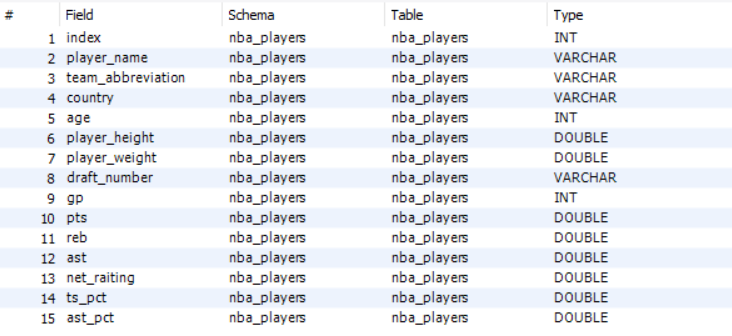
\includegraphics[width=14cm]{mysql_tables.png}
    \caption{Nazwy kolumn (atrybutów) w systemie zarządzania bazami danych MySQL}
    \label{rysunek:baza_danych}
\end{figure}

\section{Atrybuty i liczności obiektów wyrażone zmiennymi lingwistycznymi}
\subsection{Zmienne lingwistyczne}
Definicja zmiennej lingwistycznej została już wprowadzona w sekcji 1. W bieżącej sekcji skupimy się dokładniej na tej definicji podając dla każdego z 11 atrybutów z sekcji 1 nazwę zmiennej lingwistycznej, zbiór terminów lingwistycznych oraz przestrzeń rozważań. Uważamy, że podając konkretny zbiór terminów lingwistycznych, jaki wykorzystamy, reguły gramatyczna oraz semantyczna będą widoczne i nie ma potrzeby podawania ich wprost. Wszak np. dla wzrostu nie podamy jako termin lingwistyczny słowa \textit{zielony} lub \textit{szybki} oraz wszystkie terminy we wszystkich zmiennych będą uporządkowane w sposób semantyczny (np. słowo \textit{ciężki} nie wystąpi przed słowem \textit{lekki}, a słowo \textit{idealny} przed \textit{fatalny}). Poniżej przedstawiamy wykorzystane zmienne lingwistyczne wraz ze wzorami oraz wykresami:
\begin{enumerate}
    \item wiek zawodnika - przestrzeń rozważań: liczby naturalne z przedziału $[18, 44]$
    \begin{itemize}
        \item junior
        \begin{equation}
            \mu_{junior}(x) = \left\{\begin{matrix} 1 & dla \: x\in[18, 20) \wedge x\in \mathbf{N} \\ -0.25x + 6 & dla \: x\in [20, 24] \wedge x\in \mathbf{N} \\ 0 & dla \: x\in (24, 44] \wedge x\in \mathbf{N} \end{matrix}\right.
        \end{equation}
        \item młody
        \begin{equation}
            \mu_{mlody}(x) = \left\{\begin{matrix}  0 & dla \: x\in ([18, 20) \cup (28;44])  \wedge x\in \mathbf{N} \\ 0.25x-5 & dla \: x\in[20, 24) \wedge x\in \mathbf{N} \\ 1 & dla \: x\in [24, 26) \wedge x\in \mathbf{N} \\ -0.5x + 14 & dla \: x\in[26, 28] \wedge x\in \mathbf{N} \\\end{matrix}\right.
        \end{equation}
        \item w średnim wieku
        \begin{equation}
            \mu_{w srednim wieku}(x) = \left\{\begin{matrix} 0 & dla \: x\in ([18, 26) \cup (32, 44] ) \wedge x\in \mathbf{N} \\ 0.5x - 13 & dla \: x\in[26, 28) \wedge x\in \mathbf{N} \\ 1 & dla \: x\in [28, 30) \wedge x\in \mathbf{N} \\ -0.5x + 16 & dla \: x\in[30, 32] \wedge x\in \mathbf{N}  \end{matrix}\right.
        \end{equation}
        \item doświadczony
        \begin{equation}
            \mu_{doswiadczony}(x) = \left\{\begin{matrix}  0 & dla \: x\in ([18, 30) \cup  (34, 44] )  \wedge x\in \mathbf{N} \\ 0.5x - 15 & dla \: x\in[30, 32)  \wedge x\in \mathbf{N}\\ 1 & dla \: x\in [32, 34) \wedge x\in \mathbf{N} \\ -0.5x + 18 & dla \: x\in[34, 36]  \wedge x\in \mathbf{N} \end{matrix}\right.
        \end{equation}
        \item stary
        \begin{equation}
            \mu_{stary}(x) = \left\{\begin{matrix} 0 & dla \: x\in [18, 34)  \wedge x\in \mathbf{N} \\ 0.5x - 17 & dla \: x\in[34, 36)  \wedge x\in \mathbf{N} \\ 1 & dla \: x\in [36, 44]  \wedge x\in \mathbf{N} \end{matrix}\right.
        \end{equation}
    \end{itemize}
     \begin{figure}[H]
    \centering
    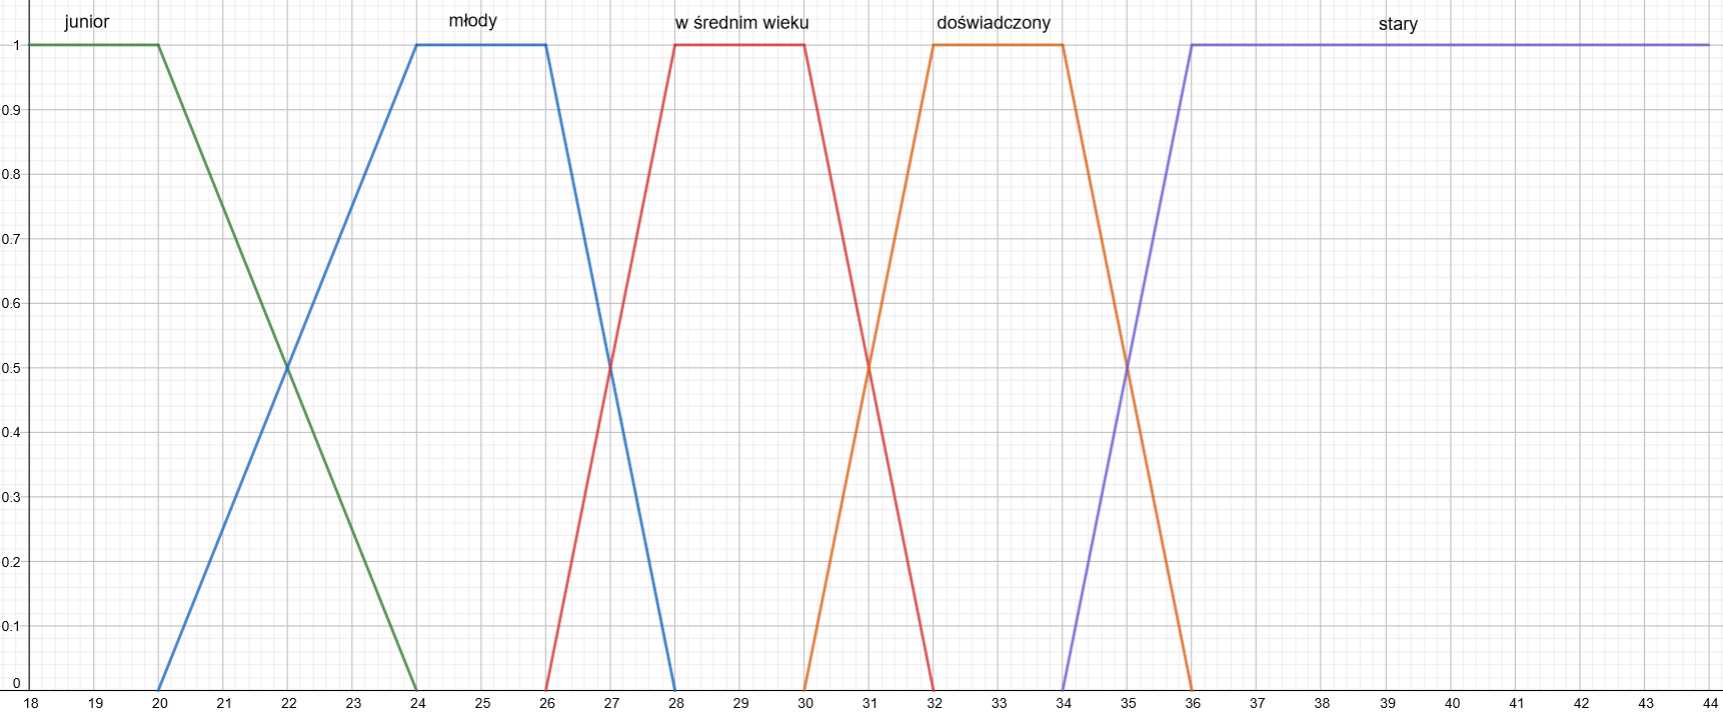
\includegraphics[width=14cm]{wykres_wiek.png}
    \caption{Wykres funkcji przynależności dla zmiennej lingwistycznej \textit{wiek zawodnika}.}
    \label{rysunek:wiek}
\end{figure}
    \item wzrost zawodnika - przestrzeń rozważań: liczby rzeczywiste z przedziału: $[160.03, 231.14]$
    \begin{itemize}
        \item niski
        \begin{equation}
            \mu_{niski}(x) = \left\{\begin{matrix} 1 & dla \: x\in[160.03, 185.0) \\ -0.1x + 19.5 & dla \: x\in [185.0, 195.0] \\ 0 & dla \: x\in (195.0, 231.14] \end{matrix}\right.
        \end{equation}
        \item średniego wzrostu
        \begin{equation}
            \mu_{sredniegowzrostu}(x) = \left\{\begin{matrix} 0 & dla \: x\in (160.03, 185.0] \cup (205.0, 231.14] \\ 0.1x - 18.5 & dla \: x\in[185.0, 195.0) \\ -0.1x + 20.5 & dla \: x\in [195.0, 205.0] \\ \end{matrix}\right.
        \end{equation}
        \item wysoki
        \begin{equation}
            \mu_{wysoki}(x) = \left\{\begin{matrix}  0 & dla \: x\in (160.03, 200.0] \\ 0.1x - 20 & dla \: x\in[200.0, 210.0) \\ 1 & dla \: x\in [210.0, 231.14] \end{matrix}\right.
        \end{equation}
        \item bardzo niski
        \begin{equation}
            \mu_{bardzoniski}(x) = \mu_{niski}(x)^2
        \end{equation}
        \item bardzo wysoki
        \begin{equation}
            \mu_{bardzowysoki}(x) = \mu_{wysoki}(x)^2
        \end{equation}
    \end{itemize}
    Oczywiście, zgodnie z regułą semantyczną termin \textit{bardzo niski} występuje przed terminem \textit{niski} w zmiennej lingwistycznej. Powyżej został on wymieniony później, ponieważ definiując funkcję przynależności dla terminu \textit{bardzo niski} korzystamy z funkcji przynależności dla terminu \textit{niski} (konkretnie podnosimy ją do kwadratu).
    \begin{figure}[H]
        \centering
        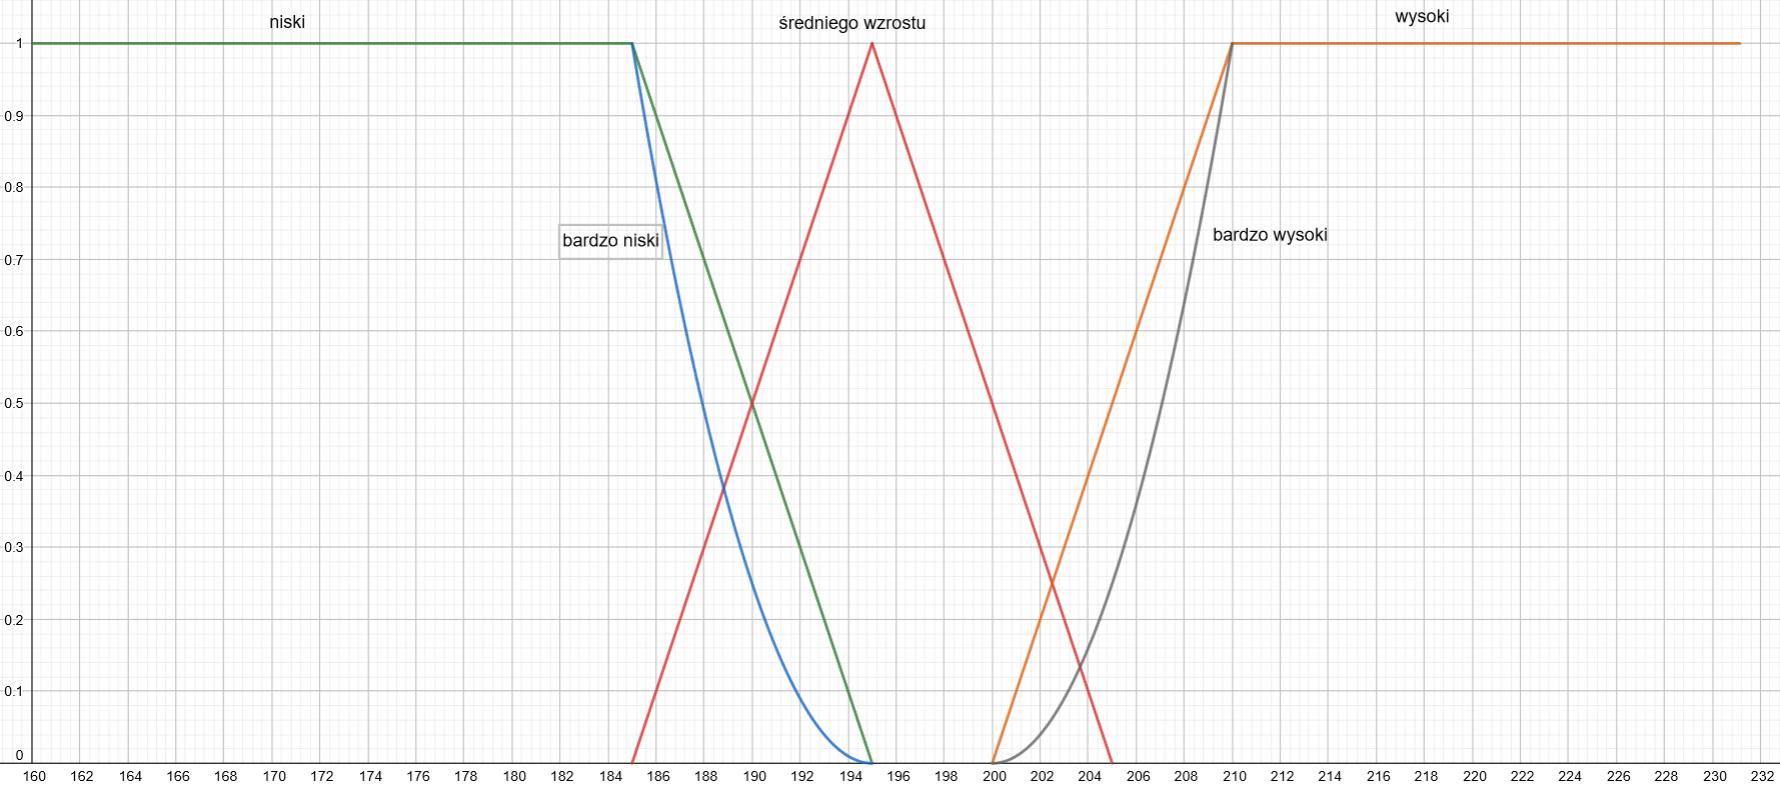
\includegraphics[width=14cm]{wykres_wzrost.png}
        \caption{Wykres funkcji przynależności dla zmiennej lingwistycznej \textit{wzrost zawodnika}.}
        \label{rysunek:wzrost}
    \end{figure}
    \item waga zawodnika - przestrzeń rozważań: Liczby rzeczywiste z przedziału: $[60.33, 163.29]$
    \begin{itemize}
        \item lekki
        \begin{equation}
            \mu_{lekki}(x) = \left\{\begin{matrix} 1 & dla \: x\in[60.33, 85.0) \\ -0.1x + 9.5 & dla \: x\in [85.0, 95.0] \\ 0 & dla \: x\in (95.0, 163.29] \end{matrix}\right.
        \end{equation}
         \item o przeciętnej wadze
        \begin{equation}
            \mu_{oprzecietnejwadze}(x) = \left\{\begin{matrix} 0 & dla \: x\in [60.33, 90.0) \cup (110.0, 163.29] \\ 0.1x - 9 & dla \: x\in[90.0, 100.0) \\ -0.1x + 11 & dla \: x\in [100.0, 110.0] \end{matrix}\right.
        \end{equation}
        \item ciężki
        \begin{equation}
            \mu_{ciezki}(x) = \left\{\begin{matrix} 0 & dla \: x\in [60.33, 105.0) \\ 0.1x - 10.5 & dla \: x\in[105.0, 115.0) \\ 1 & dla \: x\in [115.0, 163.29] \end{matrix}\right.
        \end{equation}
        \item bardzo lekki
        \begin{equation}
            \mu_{bardzolekki}(x) = \mu_{lekki}(x)^2
        \end{equation}
        \item bardzo ciężki
        \begin{equation}
            \mu_{bardzociezki}(x) = \mu_{ciezki}(x)^2
        \end{equation}
    \end{itemize}
    Oczywiście, zgodnie z regułą semantyczną termin \textit{bardzo lekki} występuje przed terminem \textit{lekki} w zmiennej lingwistycznej. Powyżej został on wymieniony później, ponieważ definiując funkcję przynależności dla terminu \textit{bardzo lekki} korzystamy z funkcji przynależności dla terminu \textit{lekki} (konkretnie podnosimy ją do kwadratu).
    \begin{figure}[H]
        \centering
        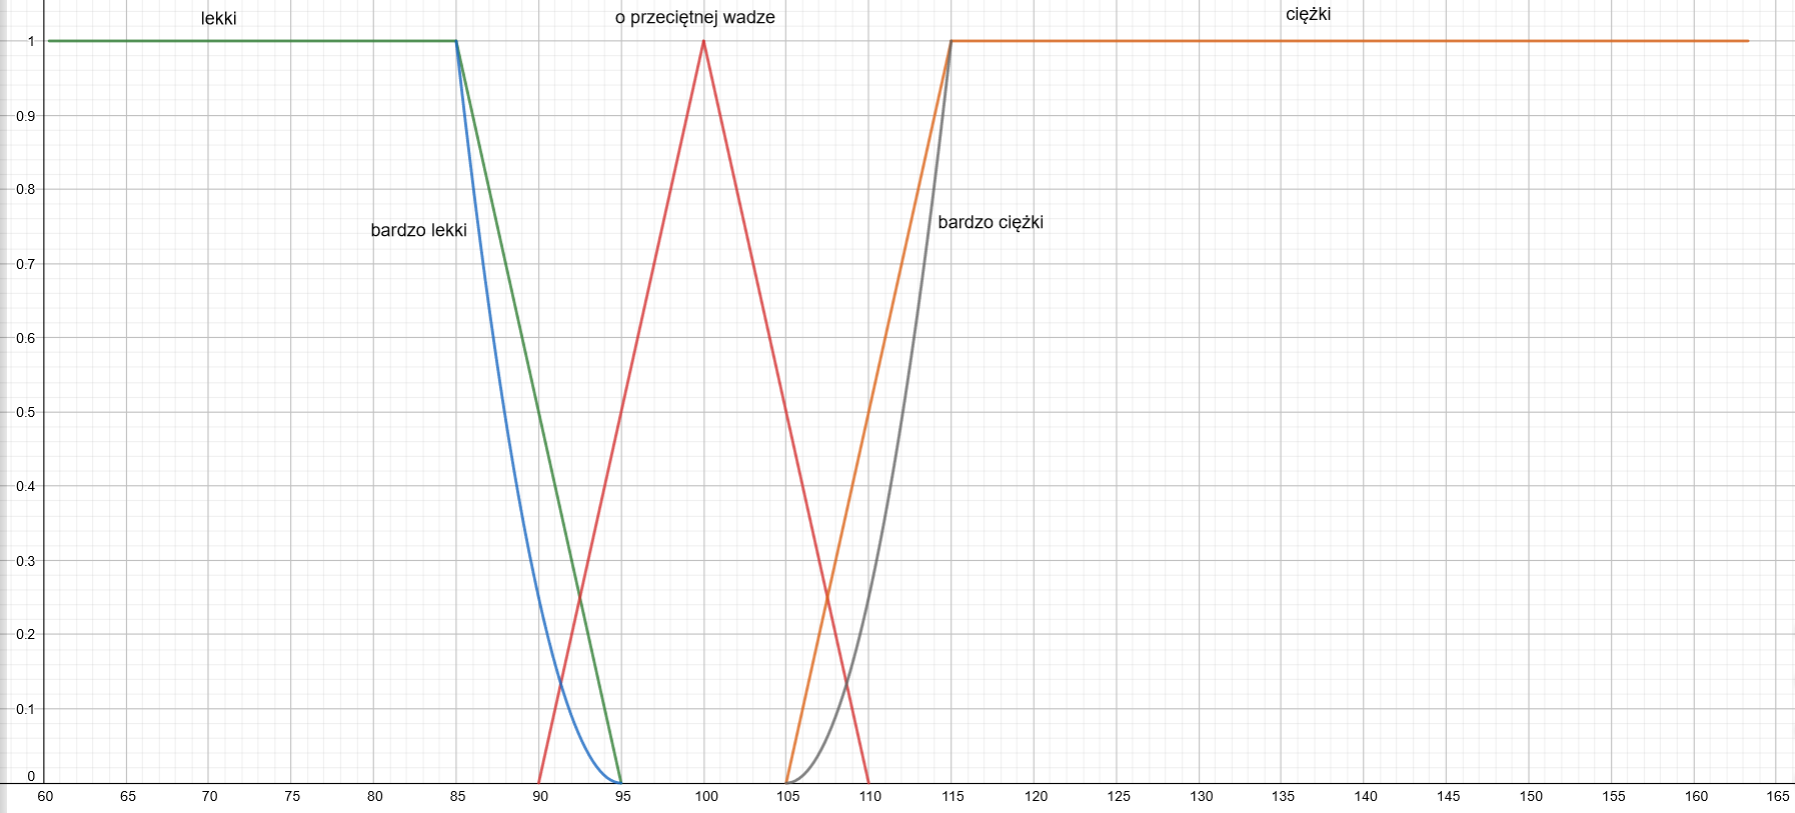
\includegraphics[width=14cm]{wykres_waga.png}
        \caption{Wykres funkcji przynależności dla zmiennej lingwistycznej \textit{waga zawodnika}.}
        \label{rysunek:waga}
    \end{figure}
    
    \item kolejność wyboru w drafcie - przestrzeń rozważań: liczby naturalne z przedziału: $[0, 60]$
    \begin{itemize}
        \item błyskawicznie
        \begin{equation}
            \mu_{blyskawicznie}(x) = \left\{\begin{matrix} 1 & dla \: x\in[0, 6) \wedge x\in \mathbf{N} \\ -0.125x + 1.75 & dla \: x\in [6, 14] \wedge x\in \mathbf{N} \\ 0 & dla \: x\in (14, 60] \wedge x\in \mathbf{N} \end{matrix}\right.
        \end{equation}
         \item szybko
        \begin{equation}
            \mu_{szybko}(x) = \left\{\begin{matrix} 0 & dla \: x\in ([0, 10) \cup (30;60]) \wedge x\in \mathbf{N} \\ 0.25x - 2.5 & dla \: x\in[10, 14) \wedge x\in \mathbf{N} \\ 1 & dla \: x\in [14, 22) \wedge x\in \mathbf{N} \\ -0.125x + 3.75 & dla \: x\in [22, 30] \wedge x\in \mathbf{N} \end{matrix}\right.
        \end{equation}
        \item średnio
        \begin{equation}
            \mu_{srednio\_draft}(x) = \left\{\begin{matrix} 0 & dla \: x\in ([0, 20) \cup (40, 60]) \wedge x\in \mathbf{N} \\ 0.1x - 2 & dla \: x\in[20, 30) \wedge x\in \mathbf{N} \\ -0.1x + 4 & dla \: x\in [30, 40] \wedge x\in \mathbf{N} \end{matrix}\right.
        \end{equation}
        \item późno
        \begin{equation}
            \mu_{pozno}(x) = \left\{\begin{matrix} 0 & dla \: x\in ([0, 36) \cup (56, 60]) \wedge x\in \mathbf{N} \\ 0.125x - 4.5 & dla \: x\in[36, 44) \wedge x\in \mathbf{N} \\ 1 & dla \: x\in [44, 48) \wedge x\in \mathbf{N} \\ -0.125x + 7 & dla \: x\in [48, 56] \wedge x\in \mathbf{N} \end{matrix}\right.
        \end{equation}
        \item na koniec
        \begin{equation}
            \mu_{nakoniec}(x) = \left\{\begin{matrix}  0 & dla \: x\in [0, 51) \wedge x\in \mathbf{N} \\ 0.2x - 10.2 & dla \: x\in[51, 56)\wedge x\in \mathbf{N} \\ 1 & dla \: x\in [56, 60]\wedge x\in \mathbf{N} \end{matrix}\right.
        \end{equation}
    \end{itemize}
    \begin{figure}[H]
        \centering
        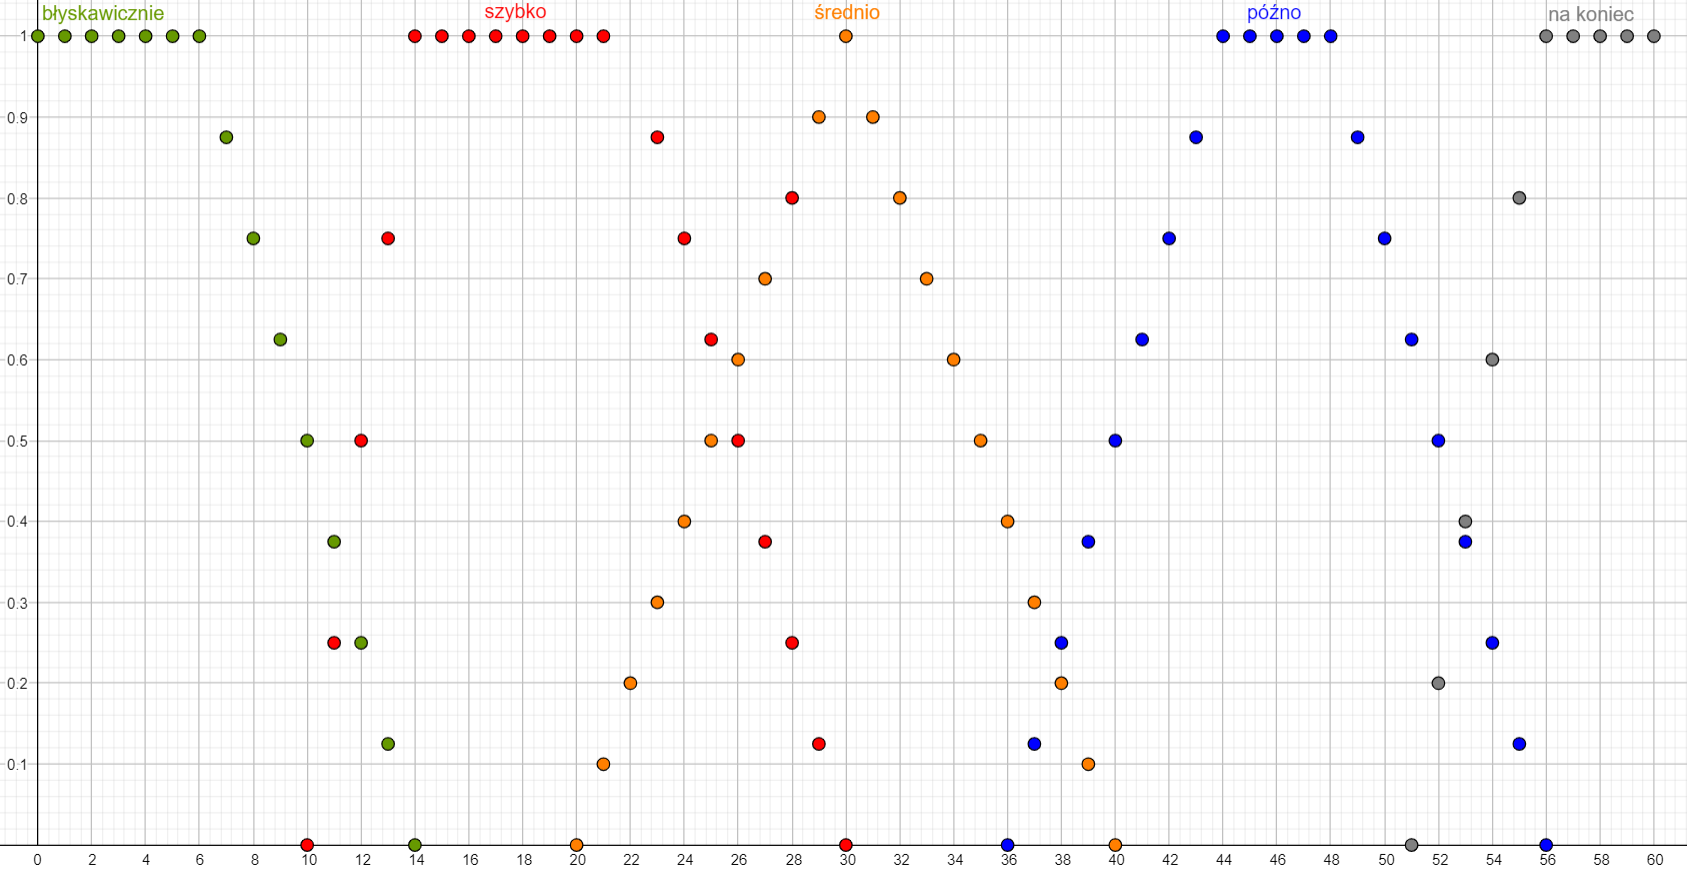
\includegraphics[width=14cm]{wykres_draft.png}
        \caption{Wykres funkcji przynależności dla zmiennej lingwistycznej \textit{kolejność wyboru w drafcie}.}
        \label{rysunek:draft}
    \end{figure}
    
    \item rozegrane gry w sezonie - przestrzeń rozważań: liczby naturalne z przedziału: $[1, 85]$
     \begin{itemize}
        \item znikoma liczba
        \begin{equation}
            \mu_{znikomaliczba}(x) = \left\{\begin{matrix} 1 & dla \: x\in[1, 10)  \wedge x\in \mathbf{N} \\ -0.0625x + 1.625 & dla \: x\in [10, 26]  \wedge x\in \mathbf{N} \\ 0 & dla \: x\in (26, 85]  \wedge x\in \mathbf{N} \end{matrix}\right.
        \end{equation}
        \item mało
        \begin{equation}
            \mu_{malo\_gier}(x) = \left\{\begin{matrix}0 & dla \: x\in ([1, 20) \cup (40;85]) \wedge x\in \mathbf{N} \\ 0.1x - 2 & dla \: x\in[20, 30) \wedge x\in \mathbf{N} \\ -0.1x + 4 & dla \: x\in [30, 40] \wedge x\in \mathbf{N}\\ \end{matrix}\right.
        \end{equation}
        \item średnio
        \begin{equation}
            \mu_{srednio\_gier}(x) = \left\{\begin{matrix} 0 & dla \: x\in ([1, 30) \cup (62, 85]) \wedge x\in \mathbf{N} \\ 0.0625x - 1.875 & dla \: x\in[30, 46) \wedge x\in \mathbf{N} \\ -0.0625x + 3.875 & dla \: x\in [46, 62] \wedge x\in \mathbf{N} \end{matrix}\right.
        \end{equation}
        \item dużo
        \begin{equation}
            \mu_{duzo\_gier}(x) = \left\{\begin{matrix} 0 & dla \: x\in ([1, 49) \cup (81, 85])  \wedge x\in \mathbf{N} \\ 0.0625x - 3.0625 & dla \: x\in[49, 65) \wedge x\in \mathbf{N} \\ -0.0625x + 5.0625 & dla \: x\in [65, 81] \wedge x\in \mathbf{N} \end{matrix}\right.
        \end{equation}
        \item maksymalnie
        \begin{equation}
            \mu_{maksymalnie}(x) = \left\{\begin{matrix} 0 & dla \: x\in [1, 70) \wedge x\in \mathbf{N} \\ 0.1x - 7 & dla \: x\in[70, 80) \wedge x\in \mathbf{N} \\ 1 & dla \: x\in [80, 85] \wedge x\in \mathbf{N} \end{matrix}\right.
        \end{equation}
    \end{itemize}
    \begin{figure}[H]
        \centering
        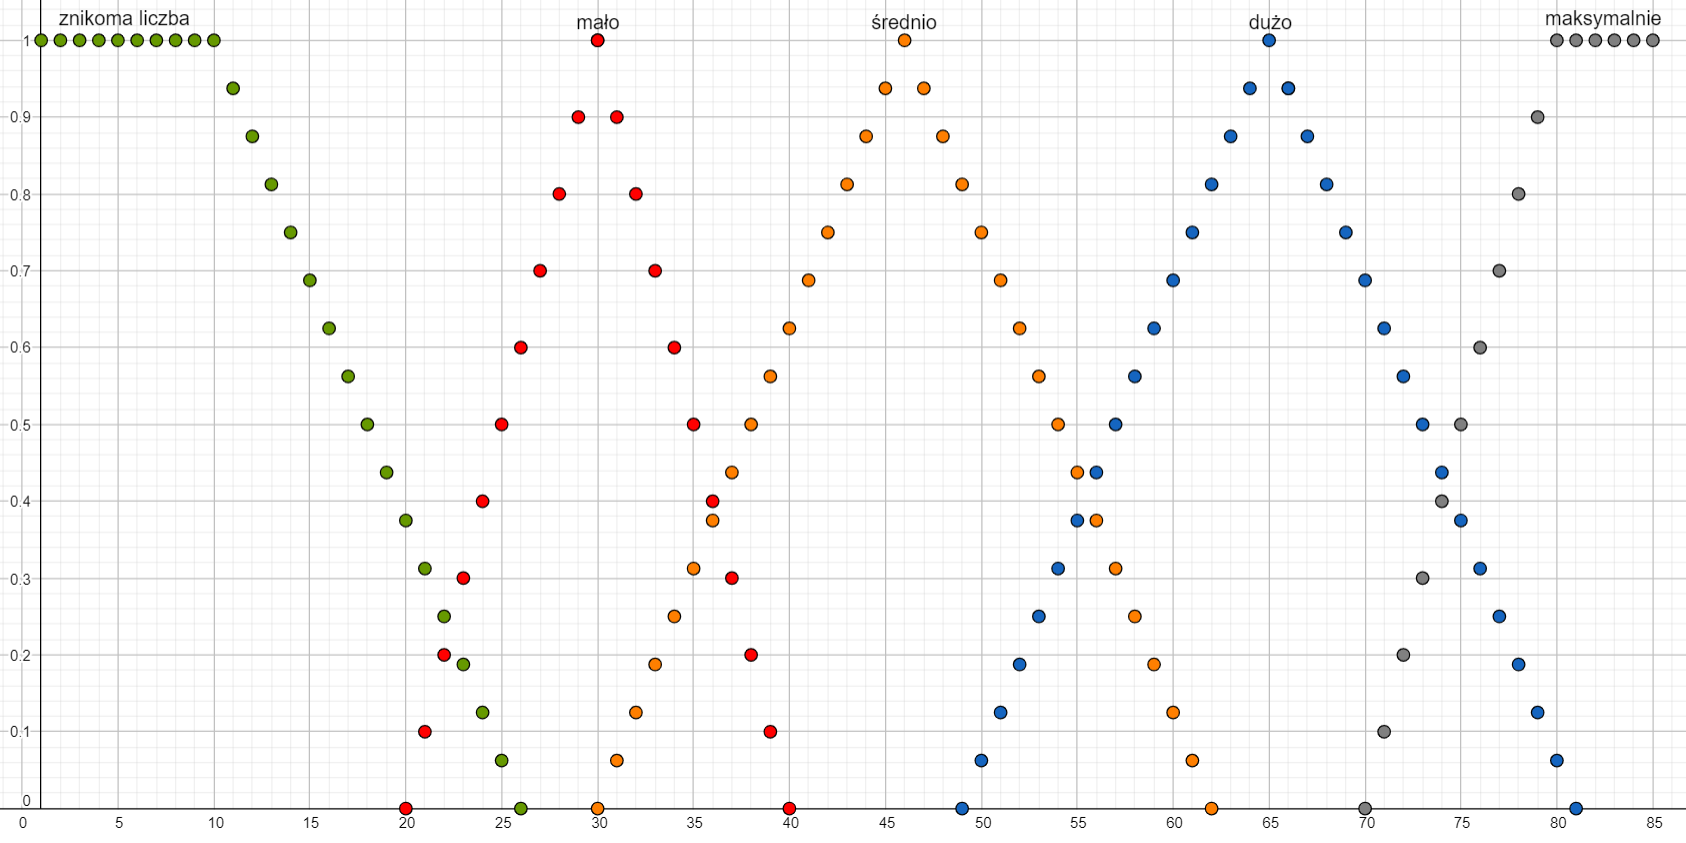
\includegraphics[width=14cm]{wykres_gry.png}
        \caption{Wykres funkcji przynależności dla zmiennej lingwistycznej \textit{rozegrane gry}.}
        \label{rysunek:gry}
    \end{figure}
    
    \item średnia liczba zdobytych punktów na mecz - przestrzeń rozważań: liczby rzeczywiste z przedziału: $[0.0, 36.1]$
    \begin{itemize}
        \item mało
        \begin{equation}
            \mu_{malo\_punktow}(x) = \left\{\begin{matrix} 1 & dla \: x\in[0.0, 1.0) \\ -0.1x + 1.1 & dla \: x\in [1.0, 11.0] \\ 0 & dla \: x\in (11.0, 36.1] \end{matrix}\right.
        \end{equation}
         \item dostatecznie
        \begin{equation}
            \mu_{dostatecznie\_punktow}(x) = \left\{\begin{matrix} 0 & dla \: x\in [0.0, 1.0) \cup (16.0, 36.0]  \\ 0.2x - 0.2 & dla \: x\in[1.0, 6.0) \\ 1 & dla \: x\in [6.0, 10.0) \\ -0.125x + 2.25 & dla \: x\in [10.0, 16.0] \end{matrix}\right.
        \end{equation}
        \item dużo
        \begin{equation}
            \mu_{duzo\_punktow}(x) = \left\{\begin{matrix}0 & dla \: x\in [0.0, 11.0) \\ 0.125x - 1.375 & dla \: x\in[11.0, 19.0) \\ 1 & dla \: x\in [19.0, 36.1] \end{matrix}\right.
        \end{equation}
        \item bardzo mało
        \begin{equation}
            \mu_{bardzomalo\_punktow}(x) = \mu_{malo}(x)^2
        \end{equation}
        \item bardzo dużo
        \begin{equation}
            \mu_{bardzoduzo\_punktow}(x) = \mu_{duzo}(x)^2
        \end{equation}
    \end{itemize}
    Oczywiście, zgodnie z regułą semantyczną termin \textit{bardzo mało} występuje przed terminem \textit{mało} w zmiennej lingwistycznej. Powyżej został on wymieniony później, ponieważ definiując funkcję przynależności dla terminu \textit{bardzo mało} korzystamy z funkcji przynależności dla terminu \textit{mało} (konkretnie podnosimy ją do kwadratu).
    \begin{figure}[H]
        \centering
        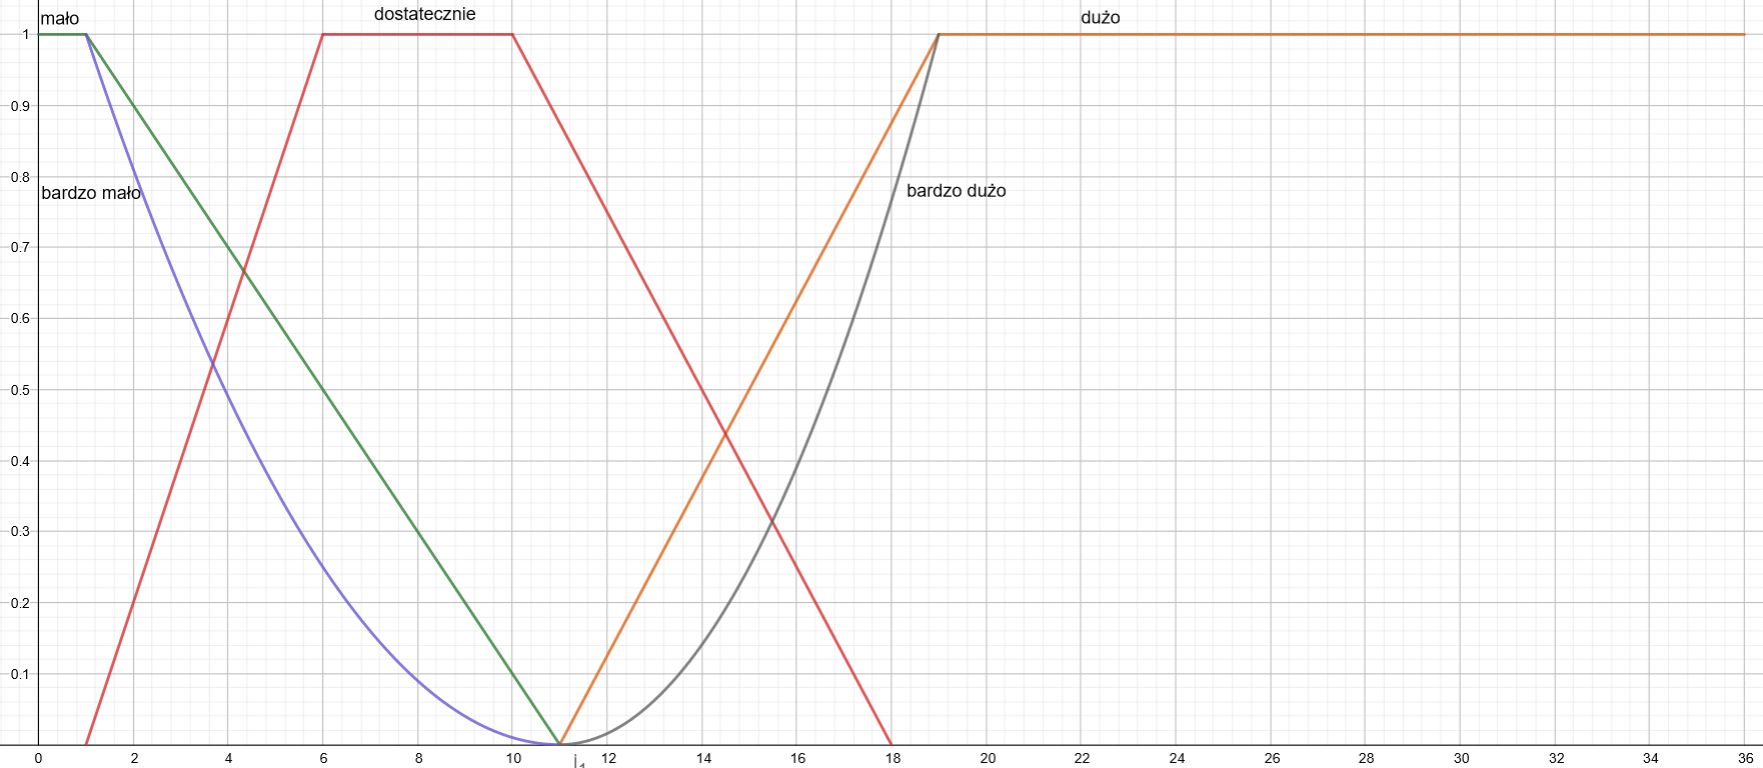
\includegraphics[width=14cm]{wykres_punkty.png}
        \caption{Wykres funkcji przynależności dla zmiennej lingwistycznej \textit{zdobyte punkty}.}
        \label{rysunek:punkty}
    \end{figure}
    
    \item średnia liczba zbiórek na mecz - przestrzeń rozważań: liczby rzeczywiste z przedziału: $[0.0, 16.3]$
    \begin{itemize}
        \item mało
        \begin{equation}
            \mu_{malo\_zbiorek}(x) = \left\{\begin{matrix} 1 & dla \: x\in[0.0, 1.0) \\ -0.25x + 1.25 & dla \: x\in [1.0, 5.0] \\ 0 & dla \: x\in (5.0, 16.3] \end{matrix}\right.
        \end{equation}
         \item dostatecznie
        \begin{equation}
            \mu_{dostatecznie\_zbiorek}(x) = \left\{\begin{matrix}0 & dla \: x\in [0.0, 2.0) \cup (6.0, 16.3] \\ 0.5x - 1 & dla \: x\in[2.0, 4.0) \\ 1 & dla \: x\in [4.0, 5.0) \\ -x + 6 & dla \: x\in [5.0, 6.0] \end{matrix}\right.
        \end{equation}
        \item dużo
        \begin{equation}
            \mu_{duzo\_zbiorek}(x) = \left\{\begin{matrix} 0 & dla \: x\in [0.0, 4.0) \\ 0.4x - 1.6 & dla \: x\in[4.0, 6.5) \\ 1 & dla \: x\in [6.5,  16.3] \end{matrix}\right.
        \end{equation}
        \item bardzo mało
        \begin{equation}
            \mu_{bardzomalo\_zbiorek}(x) = \mu_{malo}(x)^2
        \end{equation}
        \item bardzo dużo
        \begin{equation}
            \mu_{bardzoduzo\_zbiorek}(x) = \mu_{duzo}(x)^2
        \end{equation}
    \end{itemize}
    Oczywiście, zgodnie z regułą semantyczną termin \textit{bardzo mało} występuje przed terminem \textit{mało} w zmiennej lingwistycznej. Powyżej został on wymieniony później, ponieważ definiując funkcję przynależności dla terminu \textit{bardzo mało} korzystamy z funkcji przynależności dla terminu \textit{mało} (konkretnie podnosimy ją do kwadratu).
    \begin{figure}[H]
        \centering
        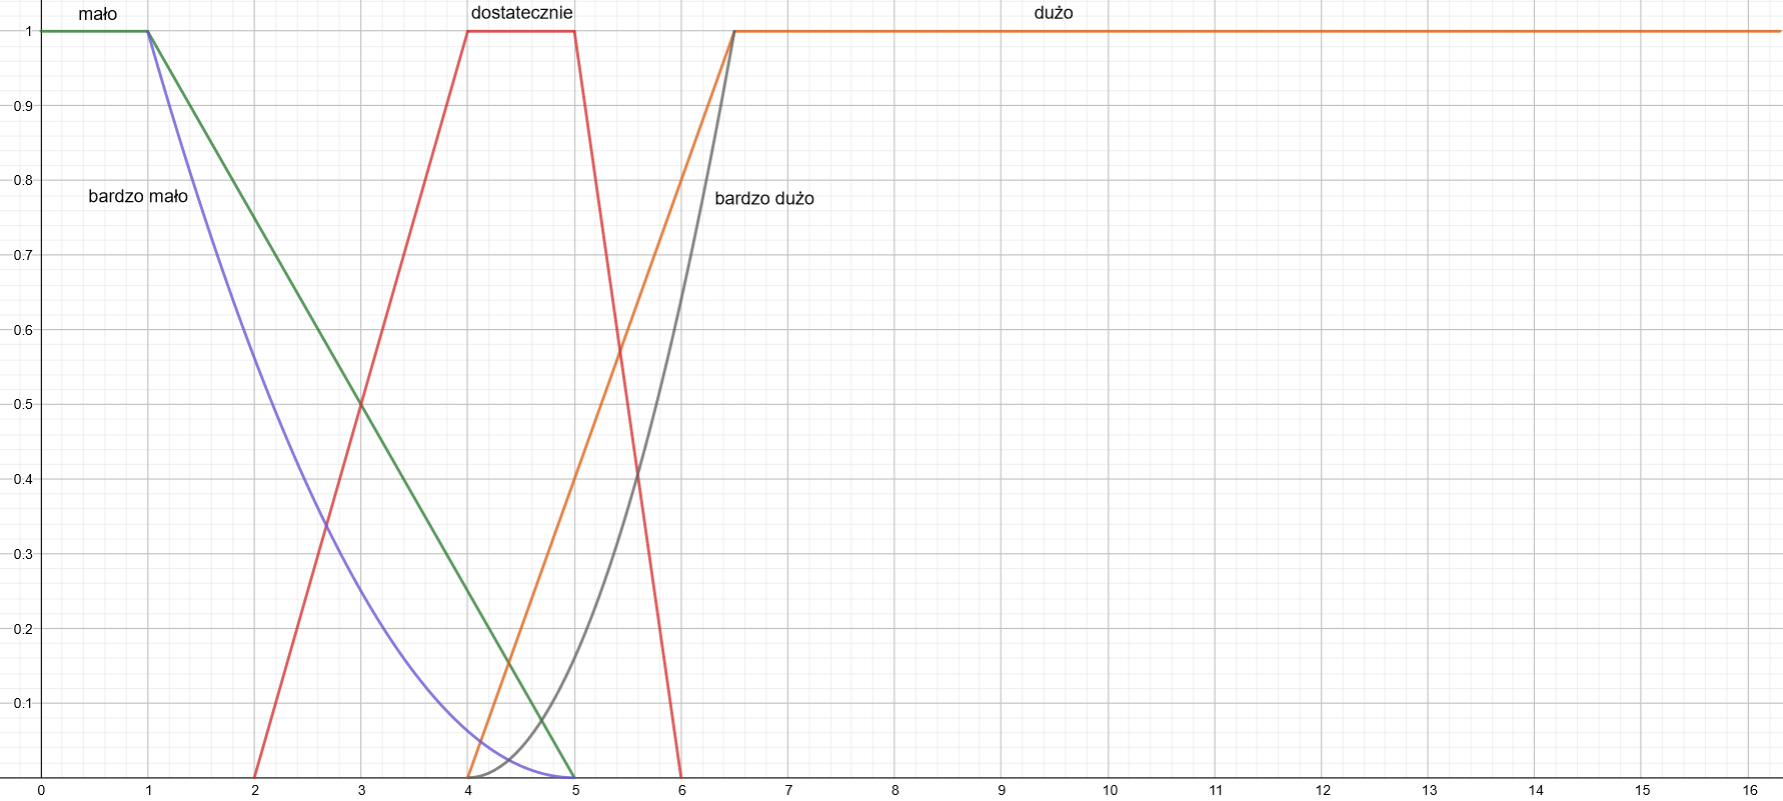
\includegraphics[width=14cm]{wykres_zbiorki.png}
        \caption{Wykres funkcji przynależności dla zmiennej lingwistycznej \textit{liczba zbiórek}.}
        \label{rysunek:zbiorki}
    \end{figure}
    
    \item średnia liczba asyst na mecz - przestrzeń rozważań: liczby rzeczywiste z przedziału: $[0.0, 11.7]$
    \begin{itemize}
        \item mało
        \begin{equation}
            \mu_{malo\_asyst}(x) = \left\{\begin{matrix} 1 & dla \: x\in[0.0, 0.5) \\ -x + 1.5 & dla \: x\in [0.5, 1.5] \\ 0 & dla \: x\in (1.5,  11.7] \end{matrix}\right.
        \end{equation}
         \item dostatecznie
        \begin{equation}
            \mu_{dostatecznie\_asyst}(x) = \left\{\begin{matrix}0 & dla \: x\in [0.0, 0.5) \cup (3.0, 11.7]\\ x - 0.5 & dla \: x\in[0.5, 1.5) \\ 1 & dla \: x\in [1.5, 2.0) \\ -x + 3 & dla \: x\in [2.0, 3.0] \end{matrix}\right.
        \end{equation}
        \item dużo
        \begin{equation}
            \mu_{duzo\_asyst}(x) = \left\{\begin{matrix}0 & dla \: x\in [0.0, 2.0) \\ 0.625x - 1.25 & dla \: x\in[2.0, 3.6) \\ 1 & dla \: x\in [3.6, 11.7] \end{matrix}\right.
        \end{equation}
        \item bardzo mało
        \begin{equation}
            \mu_{bardzomalo\_asyst}(x) = \mu_{malo\_asyst}(x)^2
        \end{equation}
        \item bardzo dużo
        \begin{equation}
            \mu_{bardzoduzo\_asyst}(x) = \mu_{duzo\_asyst}(x)^2
        \end{equation}
    \end{itemize}
    Oczywiście, zgodnie z regułą semantyczną termin \textit{bardzo mało} występuje przed terminem \textit{mało} w zmiennej lingwistycznej. Powyżej został on wymieniony później, ponieważ definiując funkcję przynależności dla terminu \textit{bardzo mało} korzystamy z funkcji przynależności dla terminu \textit{mało} (konkretnie podnosimy ją do kwadratu).
    \begin{figure}[H]
        \centering
        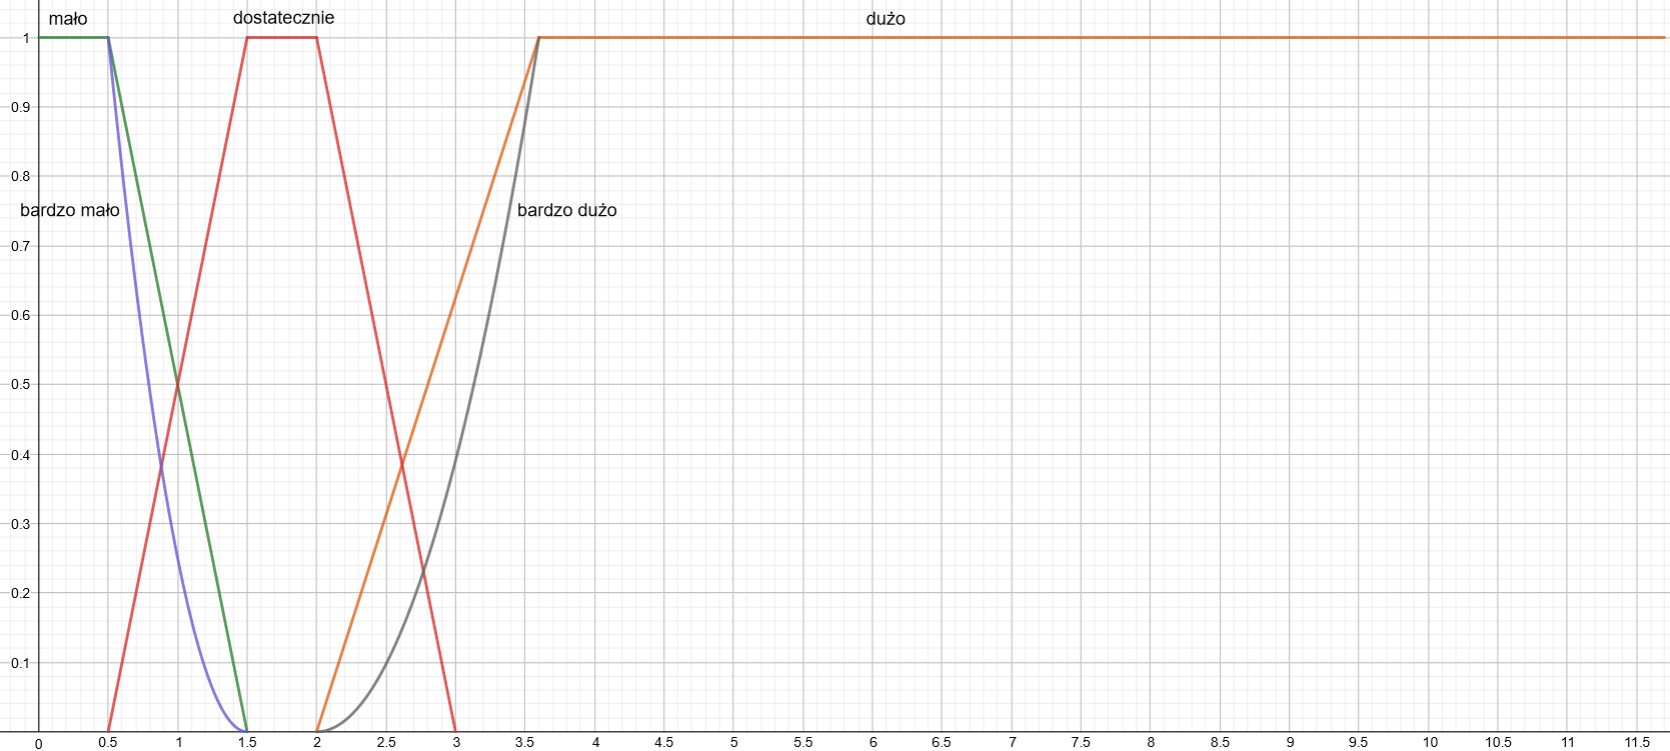
\includegraphics[width=14cm]{wykres_asysty.png}
        \caption{Wykres funkcji przynależności dla zmiennej lingwistycznej \textit{liczba asyst}.}
        \label{rysunek:asysty}
    \end{figure}
    
    \item wpływ na drużynę - przestrzeń rozważań: liczby rzeczywiste z przedziału:  $[-100.0, 100.0]$
    \begin{itemize}
        \item fatalny
        \begin{equation}
            \mu_{fatalny\_wplyw}(x) = \left\{\begin{matrix} 1 & dla \: x\in[-100.0, -15.0) \\ -0.1x - 0.5 & dla \: x\in [-15.0, -5.0] \\ 0 & dla \: x\in (-5.0, 100.0] \end{matrix}\right.
        \end{equation}
         \item negatywny
        \begin{equation}
            \mu_{negatywny\_wplyw}(x) = \left\{\begin{matrix} 0 & dla \: x\in [-100.0, -15.0) \cup (0.0, 100.0] \\ 0.125x + 1.875 & dla \: x\in[-15.0, -7.0) \\ 1 & dla \: x\in [-7.0, -2.5) \\ -0.4x & dla \: x\in [-2.5, 0.0]  \end{matrix}\right.
        \end{equation}
        \item neutralny
        \begin{equation}
            \mu_{neutralny\_wplyw}(x) = \left\{\begin{matrix} 0 & dla \: x\in [-100.0, -2.5) \cup (2.5, 100.0]  \\ 0.4x + 1 & dla \: x\in[-2.5, 0.0) \\ -0.4x + 1 & dla \: x\in [0.0, 2.5] \end{matrix}\right.
        \end{equation}
        \item pozytywny
        \begin{equation}
            \mu_{pozytywny\_wplyw}(x) = \left\{\begin{matrix} 0 & dla \: x\in [-100.0, 0.0) \cup (13.4, 100.0] \\ 0.3125x & dla \: x\in[0.0, 3.2) \\ 1 & dla \: x\in [3.2, 7.0) \\ -0.15625x + 2.09375 & dla \: x\in [7.0, 13.4]\end{matrix}\right.
        \end{equation}
        \item idealny
        \begin{equation}
            \mu_{idealny\_wplyw}(x) = \left\{\begin{matrix} 0 & dla \: x\in [-100.0, 5.0) \\ 0.125x - 0.625 & dla \: x\in[5.0, 13.0) \\ 1 & dla \: x\in [13.0, 100.0] \end{matrix}\right.
        \end{equation}
    \end{itemize}
    \begin{figure}[H]
        \centering
        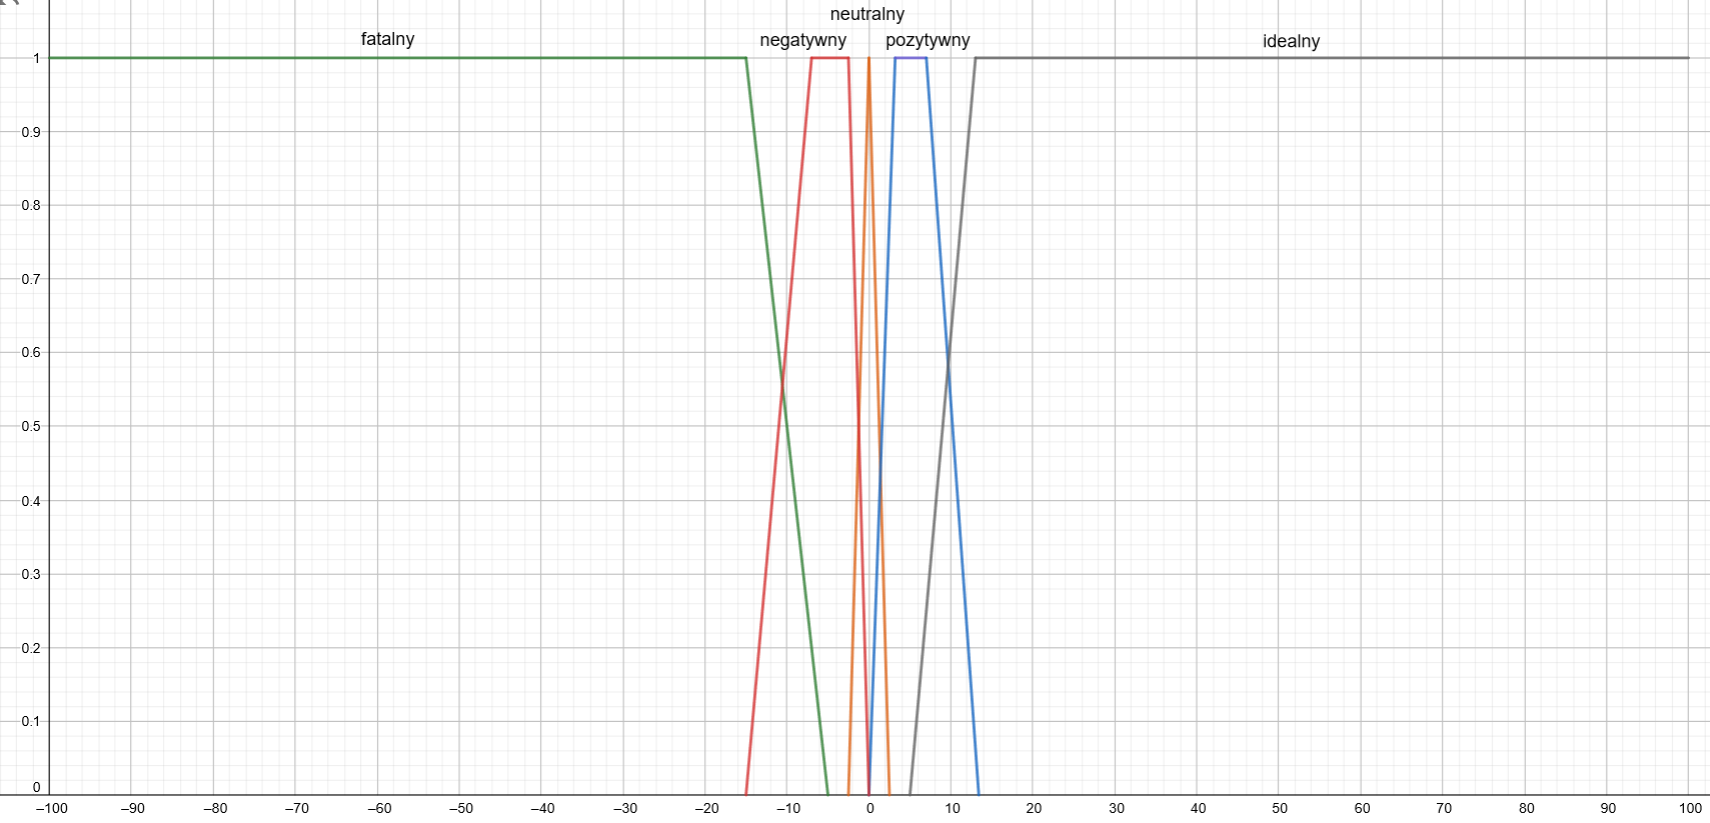
\includegraphics[width=14cm]{wykres_wplyw.png}
        \caption{Wykres funkcji przynależności dla zmiennej lingwistycznej \textit{wpływ na drużynę}.}
        \label{rysunek:wplyw}
    \end{figure}
    
    \item skuteczność rzutów - przestrzeń rozważań: liczby rzeczywiste z przedziału: $[0.0, 1.0]$
     \begin{itemize}
        \item fatalny
        \begin{equation}
            \mu_{fatalny\_skutecznosc}(x) = \left\{\begin{matrix} 1 & dla \: x\in[0.0, 0.35) \\ -10x + 4.5 & dla \: x\in [0.35, 0.45] \\ 0 & dla \: x\in (0.45, 1.0] \end{matrix}\right.
        \end{equation}
        \item nieskuteczny
        \begin{equation}
            \mu_{nieskuteczny}(x) = e^{-\frac{(x-0.4)^2}{0.003}} dla \: x \in [0.0, 1.0]
        \end{equation}
        \item przeciętny
        \begin{equation}
            \mu_{przecietny\_skutecznosc}(x) = e^{-\frac{(x-0.5)^2}{0.001}} dla \: x \in [0.0, 1.0]
        \end{equation}
        \item skuteczny
        \begin{equation}
            \mu_{skuteczny}(x) = e^{-\frac{(x-0.57)^2}{0.001}} dla \: x \in [0.0, 1.0]
        \end{equation}
        \item idealny
        \begin{equation}
            \mu_{idealny\_skutecznosc}(x) = \left\{\begin{matrix} 0 & dla \: x\in [0.0, 0.58) \\ 20x - 11.6 & dla \: x\in[0.58, 0.63) \\ 1 & dla \: x\in [0.63, 1.0] \end{matrix}\right.
        \end{equation}
    \end{itemize}
    \begin{figure}[H]
        \centering
        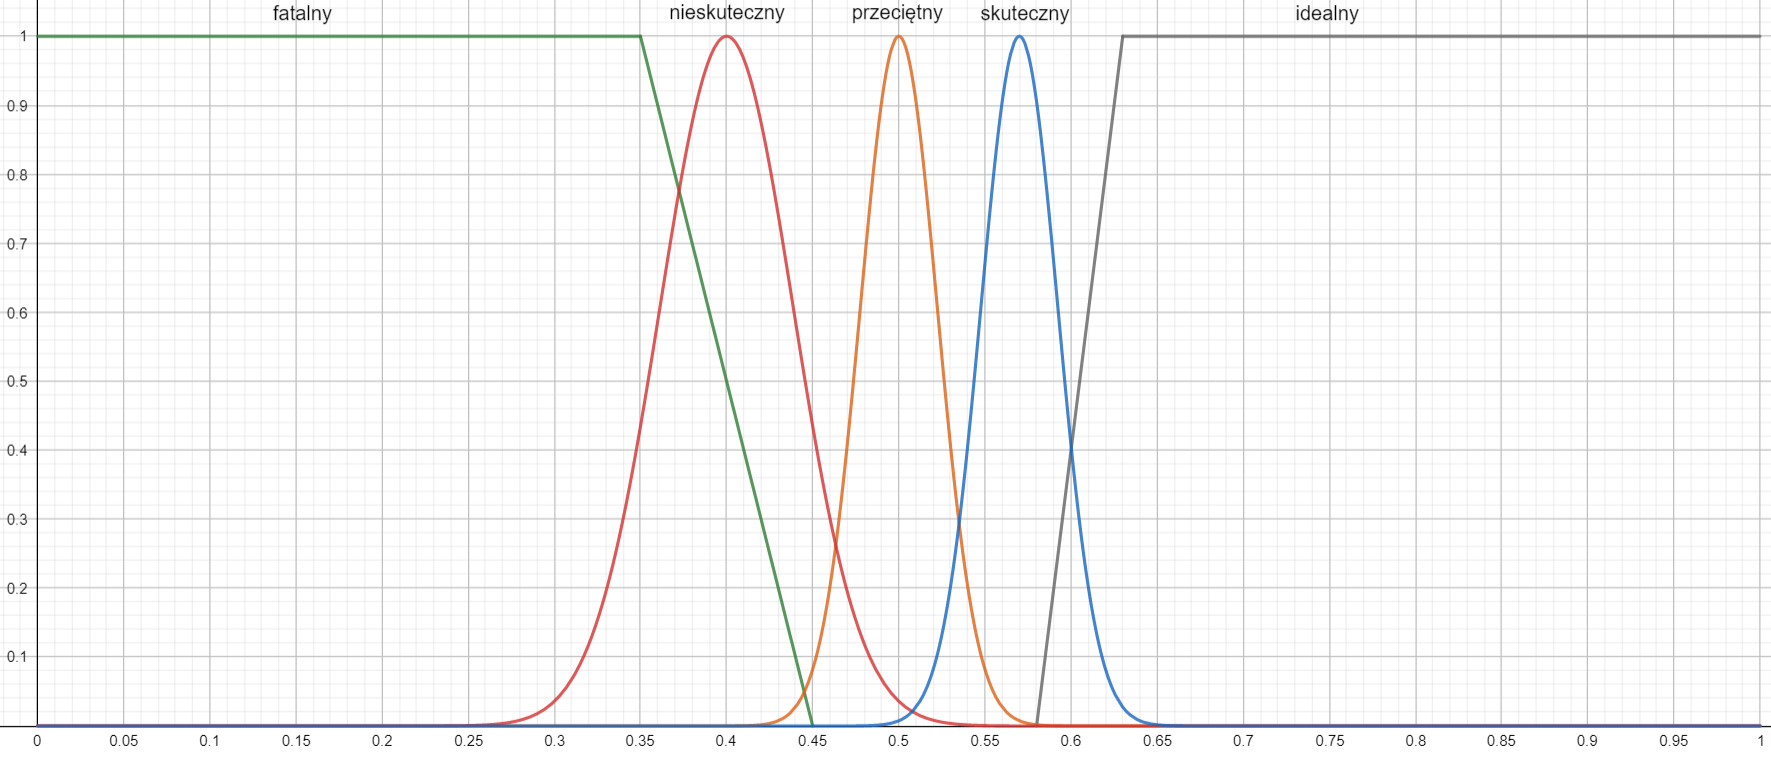
\includegraphics[width=14cm]{wykres_skutecznosc.png}
        \caption{Wykres funkcji przynależności dla zmiennej lingwistycznej \textit{skuteczność rzutów}.}
        \label{rysunek:skutecznosc}
    \end{figure}
    \item procent asyst - przestrzeń rozważań: liczby rzeczywiste z przedziału: $[0.0, 1.0]$
    \begin{itemize}
        \item fatalny
        \begin{equation}
            \mu_{fatalny\_asyst}(x) = \left\{\begin{matrix} 1 & dla \: x\in[0.0, 0.01) \\ -25x + 1.25 & dla \: x\in [0.01, 0.05] \\ 0 & dla \: x\in (0.05, 1.0] \end{matrix}\right.
        \end{equation}
        \item mały
        \begin{equation}
            \mu_{maly\_asyst}(x) = \left\{\begin{matrix} 0 & dla \: x\in [0.0, 0.01) \cup (0.06;1] \\ 25x-0.25 & dla \: x\in[0.01, 0.05) \\ 1 & dla \: x\in [0.05, 0.06) \\ -25x + 2.5 & dla \: x\in[0.06, 0.10] \end{matrix}\right.
        \end{equation}
        \item przeciętny
        \begin{equation}
            \mu_{przecietny\_asyst}(x) = \left\{\begin{matrix} 0 & dla \: x\in [0;0.06) \cup (0.19;1] \\ 12.5x - 0.75 & dla \: x\in[0.06;0.14) \\ 1 & dla \: x\in [0.14; 0.15) \\ -25x + 4.75 & dla \: x\in[0.15;0.19] \end{matrix}\right.
        \end{equation}
        \item duży
        \begin{equation}
            \mu_{duzy\_asyst}(x) = \left\{\begin{matrix} 0 & dla \: x\in [0.0, 0.15) \cup (0.31, 1.0] \\ 20x - 3 & dla \: x\in[0.15, 0.20) \\ 1 & dla \: x\in [0.20, 0.23) \\ -12.5x + 3.875 & dla \: x\in[0.23, 0.31] \end{matrix}\right.
        \end{equation}
        \item idealny
        \begin{equation}
            \mu_{idealny\_asyst}(x) = \left\{\begin{matrix} 0 & dla \: x\in [0.0, 0.23) \\ 12.5x - 2.875 & dla \: x\in[0.23, 0.31) \\ 1 & dla \: x\in [0.31, 1.0] \end{matrix}\right.
        \end{equation}
    \end{itemize}
     \begin{figure}[H]
    \centering
    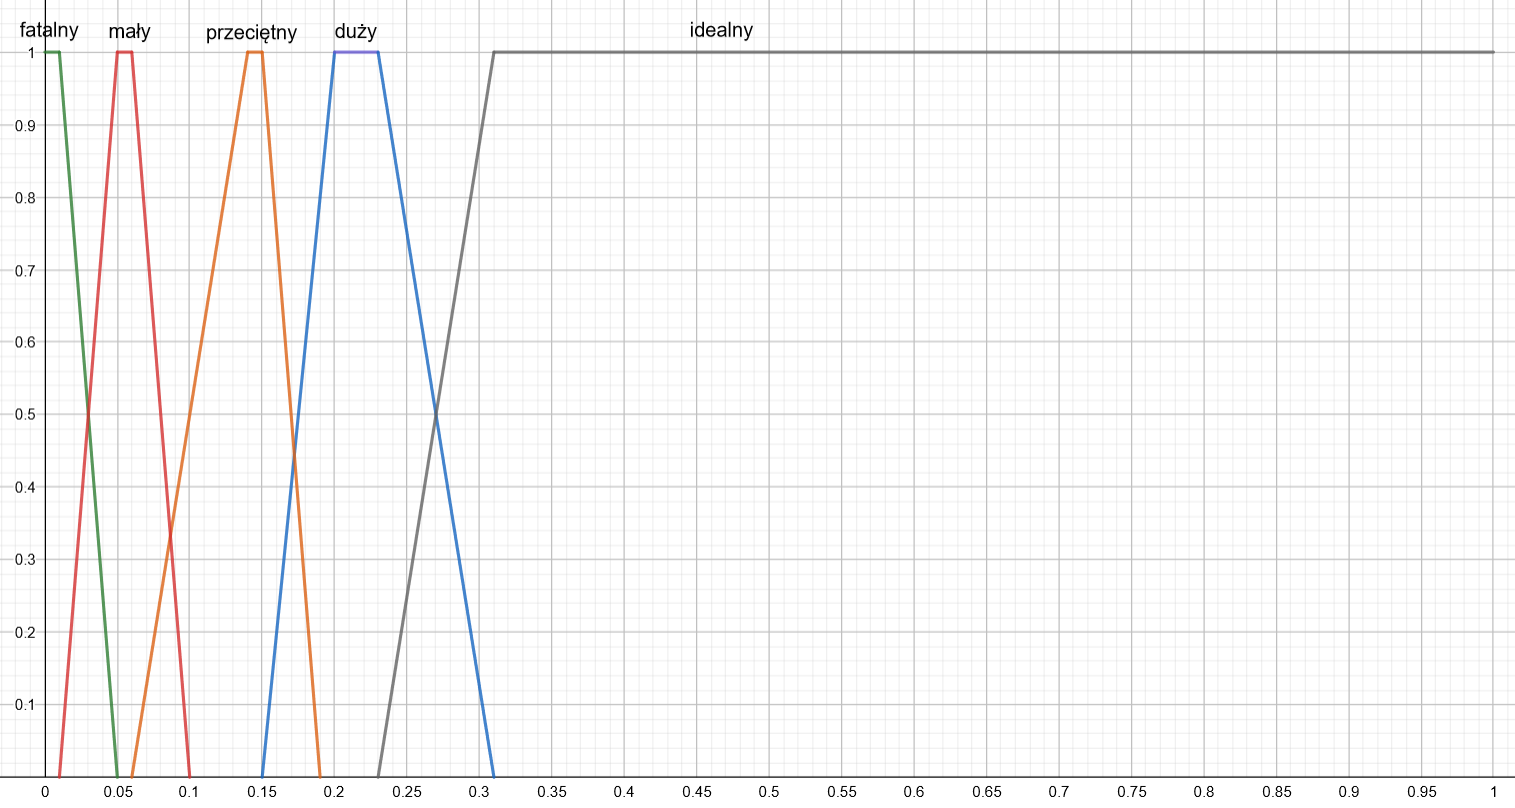
\includegraphics[width=14cm]{wykres_pr_asyst.png}
    \caption{Wykres funkcji przynależności dla zmiennej lingwistycznej \textit{procent asyst}.}
    \label{rysunek:procent_asyst}
\end{figure}
\end{enumerate}
\subsection{Kwantyfikatory lingwistyczne}
W programie zostały wykorzystane 2 typy kwantyfikatorów: absolutne oraz względne.\\
Kwantyfikatory absolutne wraz ze wzorami oraz wykresem prezentują się następująco:
\begin{itemize}
        \item Więcej niż 0
        \begin{equation}
            \mu_{wiecej\_niz\_0}(x) = \left\{\begin{matrix} -0.000667x + 1 & dla \: x\in[0, 1500] \\ 0 & dla  \: x\in (1500, 11144] \end{matrix}\right.
        \end{equation}
        \item Około 2000
        \begin{equation}
            \mu_{okolo\_2000}(x) = \left\{\begin{matrix} 0 & dla \: x\in [0;500) \\ 0.000667x - 0.333 & dla \: x\in[500;2000) \\ -0.000667x + 2.333& dla \: x\in [2000; 3500) \\ 0 & dla \: x\in[3500, 11144] \end{matrix}\right.
        \end{equation}
        \item Około 4000
        \begin{equation}
            \mu_{okolo\_4000}(x) = \left\{\begin{matrix} 0 & dla \: x\in [0, 2500) \\ 0.000667x - 1.667 & dla \: x\in[2500, 4000) \\ -0.000667x + 3.667 & dla \: x\in [4000, 5500) \\ 0 & dla \: x\in[5500, 11144] \end{matrix}\right.
        \end{equation}
        \item Około 6000
        \begin{equation}
            \mu_{okolo\_6000}(x) = \left\{\begin{matrix} 0 & dla \: x\in [0, 4500) \\ 0.000667x - 3 & dla \: x\in[4500, 6000) \\ 0.000667x + 5 & dla \: x\in [6000, 7500) \\ 0 & dla \: x\in[7500, 11144] \end{matrix}\right.
        \end{equation}
        \item Około 8000
        \begin{equation}
            \mu_{okolo\_8000}(x) = \left\{\begin{matrix} 0 & dla \: x\in [0, 6500) \\ 0.000667x - 4.333 & dla \: x\in[6500, 8000) \\ -0.000667x + 6.333 & dla \: x\in [8000, 9500) \\ 0 & dla \: x\in[9000, 11144] \end{matrix}\right.
        \end{equation}
        \item Prawie 11144
        \begin{equation}
            \mu_{prawie\_11144}(x) = \left\{\begin{matrix} 0 & dla \: x\in [0, 8500) \\ 0.000378x - 3.215 & dla \: x\in [8500, 11144] \end{matrix}\right.
        \end{equation}
    \end{itemize}
\begin{figure}[H]
    \centering
    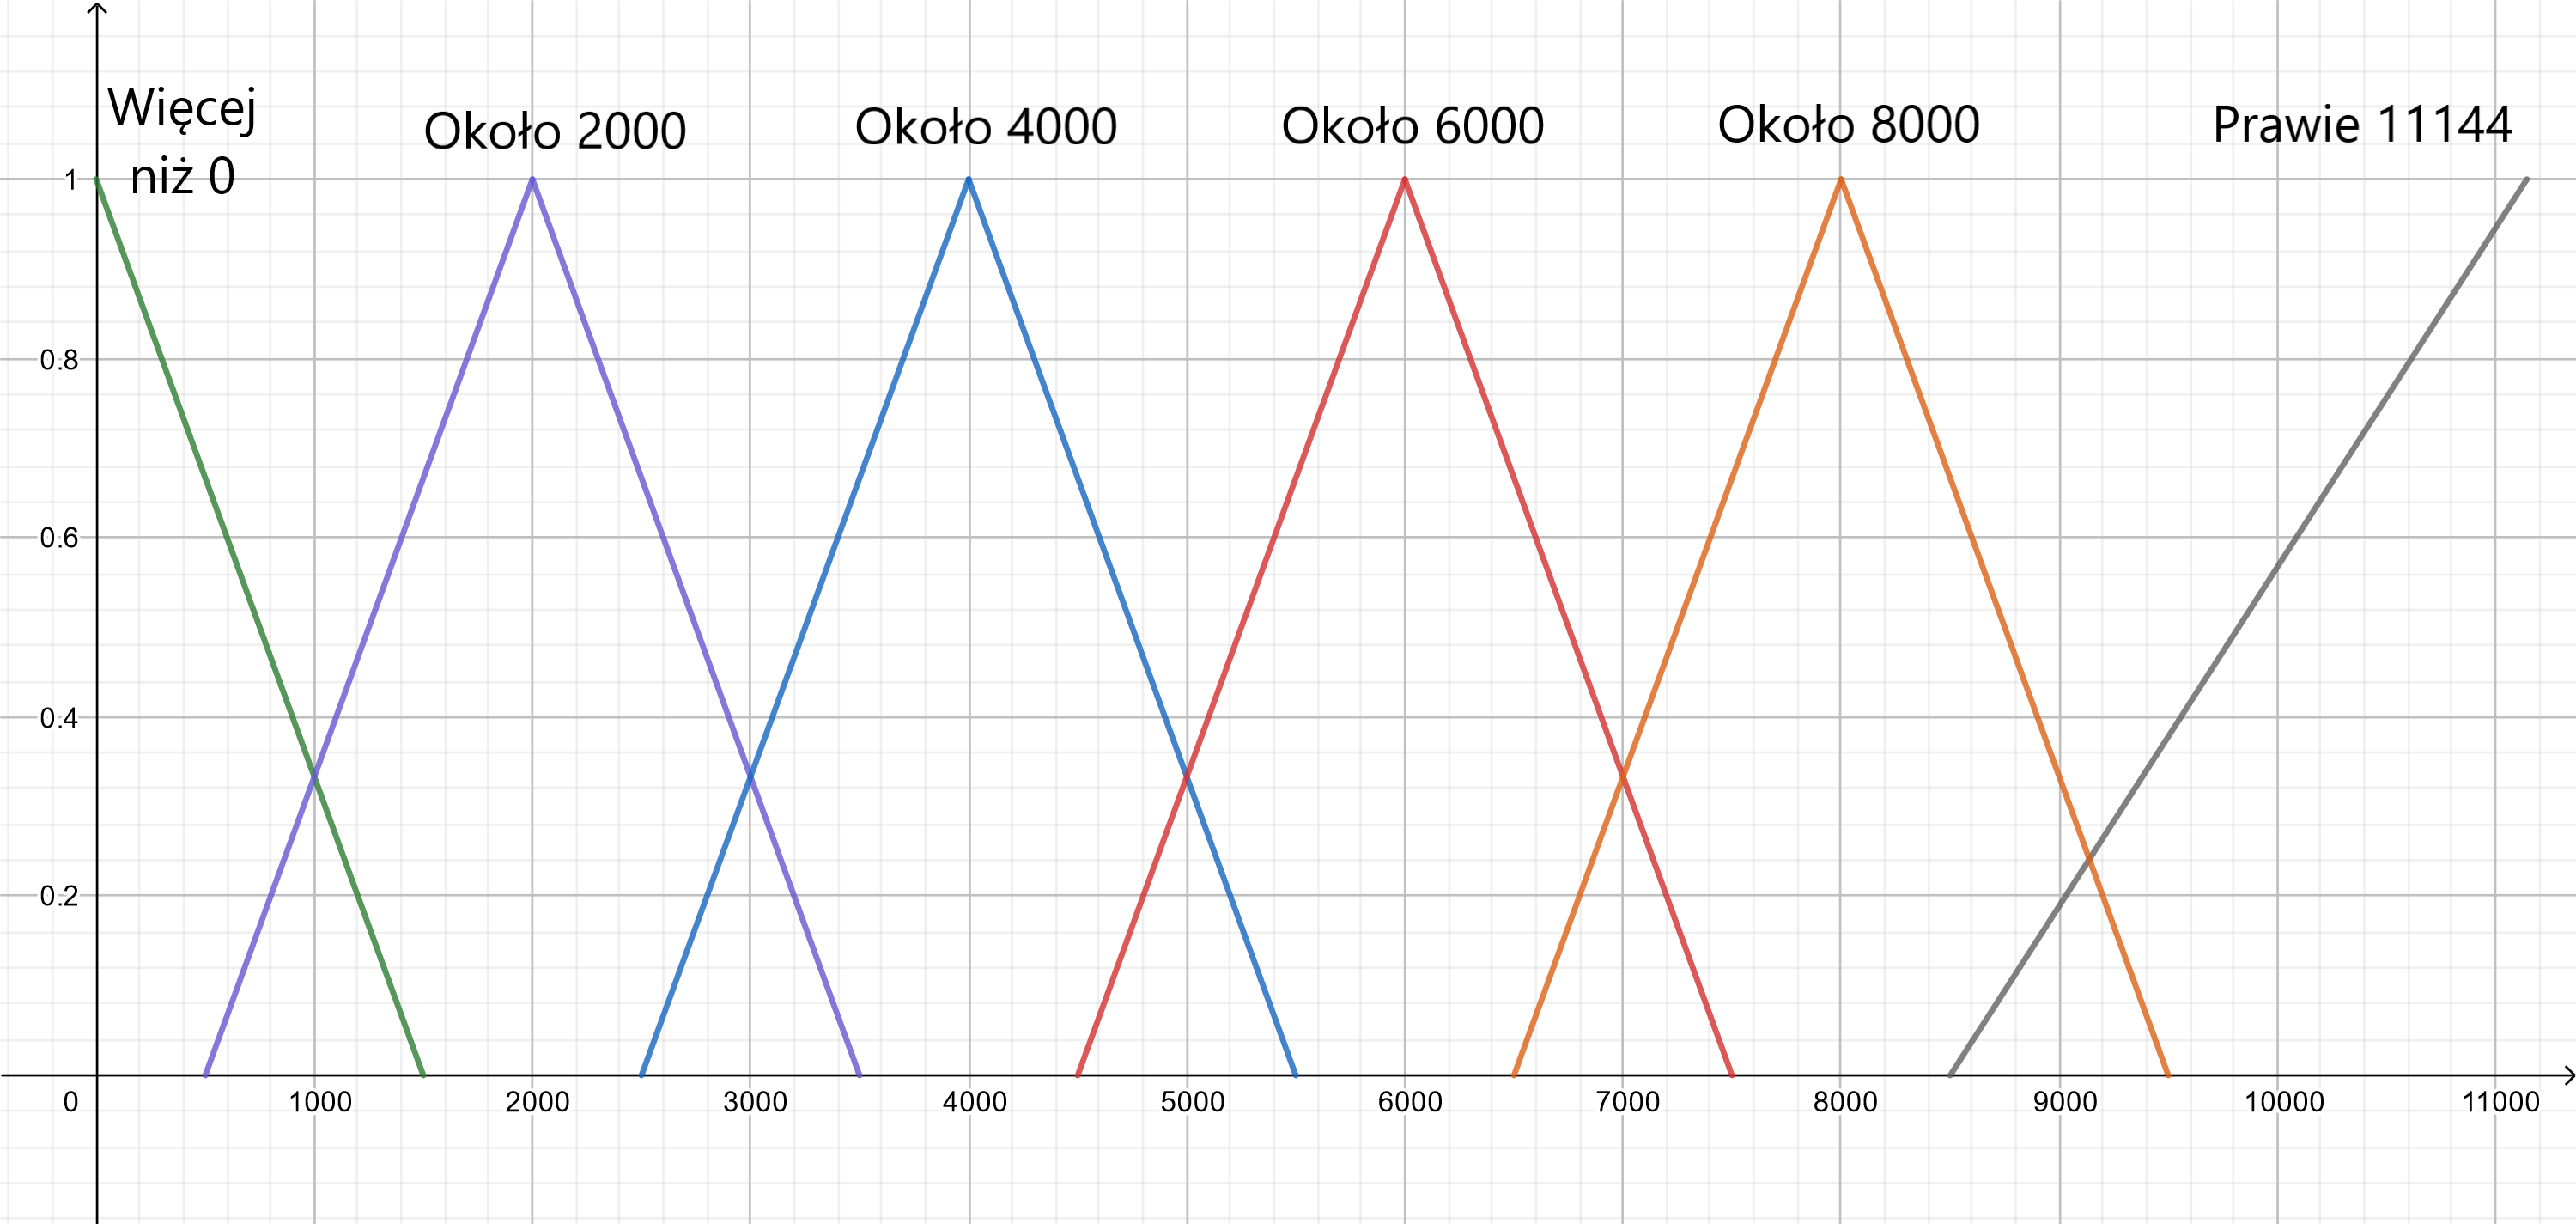
\includegraphics[width=14cm]{wykres_kwantyfikator_absolutny.png}
    \caption{Wykres funkcji przynależności dla kwantyfikatora absolutnego.}
    \label{rysunek:kwantyfikator_absolutny}
\end{figure}
Kwantyfikatory względne wraz z wzorami oraz wykresem wyglądają następująco:
\begin{itemize}
        \item Prawie żaden
        \begin{equation}
            \mu_{prawie\_zaden}(x) = \begin{matrix} e ^ {-\frac{x^2}{0.01}} & dla \: x\in [0, 1]  \end{matrix}.
        \end{equation}
        \item Około 1/4
        \begin{equation}
            \mu_{okolo\_1/4}(x) =  \begin{matrix} e ^ {-\frac{(x - 0.25)^2}{0.01}} & dla \: x\in [0, 1]  \end{matrix}.
        \end{equation}
        \item Około 1/2
        \begin{equation}
            \mu_{okolo\_1/2}(x) = \begin{matrix} e ^ {-\frac{(x - 0.5)^2}{0.01}} & dla \: x\in [0, 1]  \end{matrix}.
        \end{equation}
        \item Około 3/4
        \begin{equation}
            \mu_{okolo\_3/4}(x) = \begin{matrix} e ^ {-\frac{(x - 0.75)^2}{0.01}} & dla \: x\in [0, 1]  \end{matrix}.
        \end{equation}
        \item Prawie wszystkie
        \begin{equation}
            \mu_{prawie\_wszystkie}(x) = \begin{matrix} e ^ {-\frac{(x - 1)^2}{0.01}} & dla \: x\in [0, 1]  \end{matrix}.
        \end{equation}
    \end{itemize}
\begin{figure}[H]
    \centering
    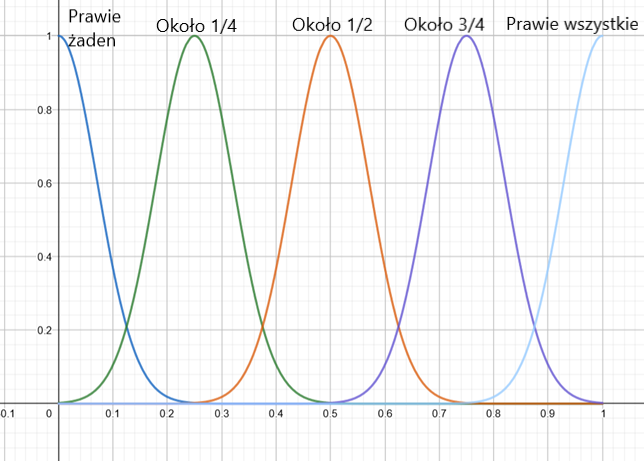
\includegraphics[width=14cm]{wykres_kwantyfikator_relatywny.png}
    \caption{Wykres funkcji przynależności dla kwantyfikatora relatywnego.}
    \label{rysunek:kwantyfikator_relatywny}
\end{figure}


\section{Narzędzia obliczeniowe: projekt (wybór, implementacja) i diagram UML pakietu obliczeń rozmytych. Diagram UML generatora podsumowań}
\subsection{Diagram pakietu obliczeń rozmytych}
Jako iż podsumowania lingwistyczne opierają się na teorii zbiorów rozmytych, na potrzeby tego zadania postanowiliśmy zaimplementować własny pakiet przeznaczony do obliczeń rozmytych. Pakiet nazywa się \textit{FuzzySetCalculations} i składa się z następujących elementów:

{\bf FuzzySet} - klasa, która reprezentuje zbiór rozmyty. 
Metody tej klasy zapewniają najbardziej istotne funkcjonalności dla podsumowań własności. 
Pierwszą z nich jest metoda o nazwie \textit{getHeight()}, która zwraca wysokość zbioru rozmytego, tj. maksymalną wartość jaką przyjmuje funkcja przynależności w całej przestrzeni rozważań.
Kolejna metoda to \textit{getSupport()}, której wynikiem wykonania są wszystkie te elementy zbioru rozmytego, które przynależą do zbioru rozmytego w stopniu większym niż 0. Bardzo podobną metodą jest \textit{getAlphaCount(double y)}, która jako argument przyjmuje wartość zbioru rozmytego. Argument ten stanowi próg dla selekcji elementów, dla których wartość funkcji przynależności jest powyżej niego. Kolejną w kolejności jest metoda \textit{getComplement(double x)}, której zadaniem jest zwrócenie dopełnienia zbioru rozmytego dla argumentu x, czyli liczby, którą trzeba dodać w celu uzyskania wartości 1. Następne dwie metody, czyli \textit{getAndResult(List<FuzzySet> fuzzySet)} i \textit{getOrResult(List<FuzzySet> fuzzySet)} odpowiadają za operacje sumy (OR) i iloczynu (AND) zbiorów rozmytych (wynikiem tych operacji również jest zbiór rozmyty). Suma zbiorów rozmytych jest obliczana jako maksimum (wykorzystanie T-normy) ze wszystkich wartości zbiorów rozmytych przekazanych w argumencie dla elementu x. Iloczyn zbiorów rozmytych jest obliczany jako minimum (wykorzystanie S-normy) ze wszystkich wartości zbiorów rozmytych przekazanych w argumencie dla wszystkich elementów w przestrzeni. Następną metodą jest metoda \textit{getDegreeOfMembership(double x)}, która dla elementu x zwraca stopień przynależności do zbioru rozmytego (w metodzie tej następuje de facto wywołanie metody \textit{countMembership(double x)} z klasy \textit{MembershipFunction}.
Kolejną metody to \textit{isConvex()} oraz \textit{isConcave()}, które zwracają wartość logiczną true w momencie, gdy zbiór rozmyty jest wypukły oraz wklęsły. Ostatnią z metod, którą planujemy zaimplementować jest metoda \textit{getCardinality()}, dzięki której otrzymujemy moc zbioru rozmytego tj. sumę wartości funkcji charakterystycznej z wszystkich elementów zbioru rozmytego. \cite{niewiadomski08}\\
{\bf MembershipFunction} - klasa abstrakcyjna, która reprezentuje funkcje przynależności do zbioru rozmytego. Klasa ta zawiera jedną metodę abstrakcyjną o nazwie \textit{countMembership(double x)}. Dzięki temu, w klasach dziedziczących można zaimplementować obliczanie stopnia przynależności w zależności od tego, jakiego rodzaju funkcji przynależności chcemy użyć. \cite{uml_doc} 
Z klasy \textit{MembershipFunction} dziedziczy pięć klas:
\begin{itemize}
    \item {\bf TrapezoidalMembershipFunction} - reprezentuje trapezoidalną funkcję przynależności. W przypadku klasy \textit{LeftTrapezoidalMembershipFunction} (funkcja malejąca) wykorzystane zostają 3 argumenty: \\
    x1 - początek przedziału od którego funkcja przyjmuje wartość 1 \\
    x2 - koniec przedziału dla którego funkcja przyjmuje wartość 1 i początek przedziału dla funkcji malejącej \\
    x3 - koniec przedziału dla funkcji malejącej i początek przedziału dla funkcji malejącej \\
    W przypadku klasy \textit{RightTrapezoidalMembershipFunction} również występują 3 argumenty: \\
    x1 - początek przedziału od którego funkcja jest rosnąca \\
    x2 - koniec przedziału dla którego funkcja jest rosnąca i początek przedziału dla funkcji stałej o wartości 1 \\
    x3 - koniec przedziału dla funkcji stałej o wartości równej 1 \\
    Do funkcjonowania klasy \textit{BothSidesTrapezoidalMembershipFunction} niezbędne są natomiast 4 argumenty: \\
    x1 - początek przedziału od którego funkcja zaczyna rosnąć \\
    x2 - koniec przedziału dla funkcji rosnącej i początek przedziału dla funkcji stałej o wartości 1 \\
    x3 - koniec przedziału dla funkcji stałej o wartości 1 i początek przedziału dla funkcji malejącej \\
    x4 - koniec przedziału dla funkcji malejącej 
    \item {\bf TriangularMembershipFunction} - reprezentuje trójkątną funkcję przynależności. Jako, że funkcja ta może być malejąca, rosnąca lub też składać się z obu tego rodzaju funkcji, w tym celu z klasy \textit{GaussianMembershipFunction} dziedziczą trzy funkcje, które reprezentują wymienione wyżej rodzaje monotoniczności. W przypadku klasy \textit{LeftTriangularMembershipFunction} (funkcja malejąca) wykorzystane zostają 3 argumenty: \\
    x1 - początek przedziału od którego funkcja zaczyna maleć \\
    x2 - koniec przedziału dla funkcji malejącej i początek przedziału dla funkcji stałej o wartości 1 \\
    W przypadku klasy \textit{RightTriangularMembershipFunction} również występują 2 argumenty:\\
    x1 - początek przedziału od którego funkcja zaczyna rosnąć \\
    x2 - koniec przedziału dla funkcji rosnącej. \\
    Do funkcjonowania klasy \textit{BothSidesTriangularMembershipFunction} niezbędne są natomiast 3 argumenty: \\
    x1 - początek przedziału od którego funkcja zaczyna rosnąć \\
    x2 - koniec przedziału dla funkcji rosnącej i początek przedziału dla funkcji stałej o wartości 1 \\
    x3 - koniec przedziału dla funkcji malejącej.
    \item {\bf ExponentialMembershipFunction} - reprezentuje wykładniczą funkcję przynależności. Jej zadaniem jest wzmocnienie/osłabienie innej funkcji przynależności (np. poprzez dodanie słowa bardzo). Argumenty, które są przez nią przyjmowane to: \\
    \textit{exponent} - wykładnik funkcji \\
    \textit{membershipFunction} - wybrana funkcja przynależności 
    \item {\bf GaussianMembershipFunction}- reprezentuje funkcję Gaussa, jako funkcję przynależności. Parametry przez nią przyjmowane to średnia oraz wariancja, które mają bezpośredni wpływ na element, gdzie znajduje się maksimum oraz na rozłożenie funkcji w dziedzinie. Jako, że funkcja ta może być malejąca, rosnąca lub też składać się z obu tego rodzaju funkcji, w tym celu z klasy \textit{GaussianMembershipFunction} dziedziczą trzy funkcje, które reprezentują wymienione wyżej rodzaje monotoniczności.
    \item {\bf BinaryMembershipFunction} - stanowi funkcję przynależności dla zbiorów klasycznych, tj. takich w których stopień przynależności do zbioru wynosi 0 lub 1. Jedynym argumentem jest \textit{rangeSet}, który to zakres określa, dla jakich elementów funkcja zwraca 1.
\end{itemize}
\begin{figure}[H]
    \centering
    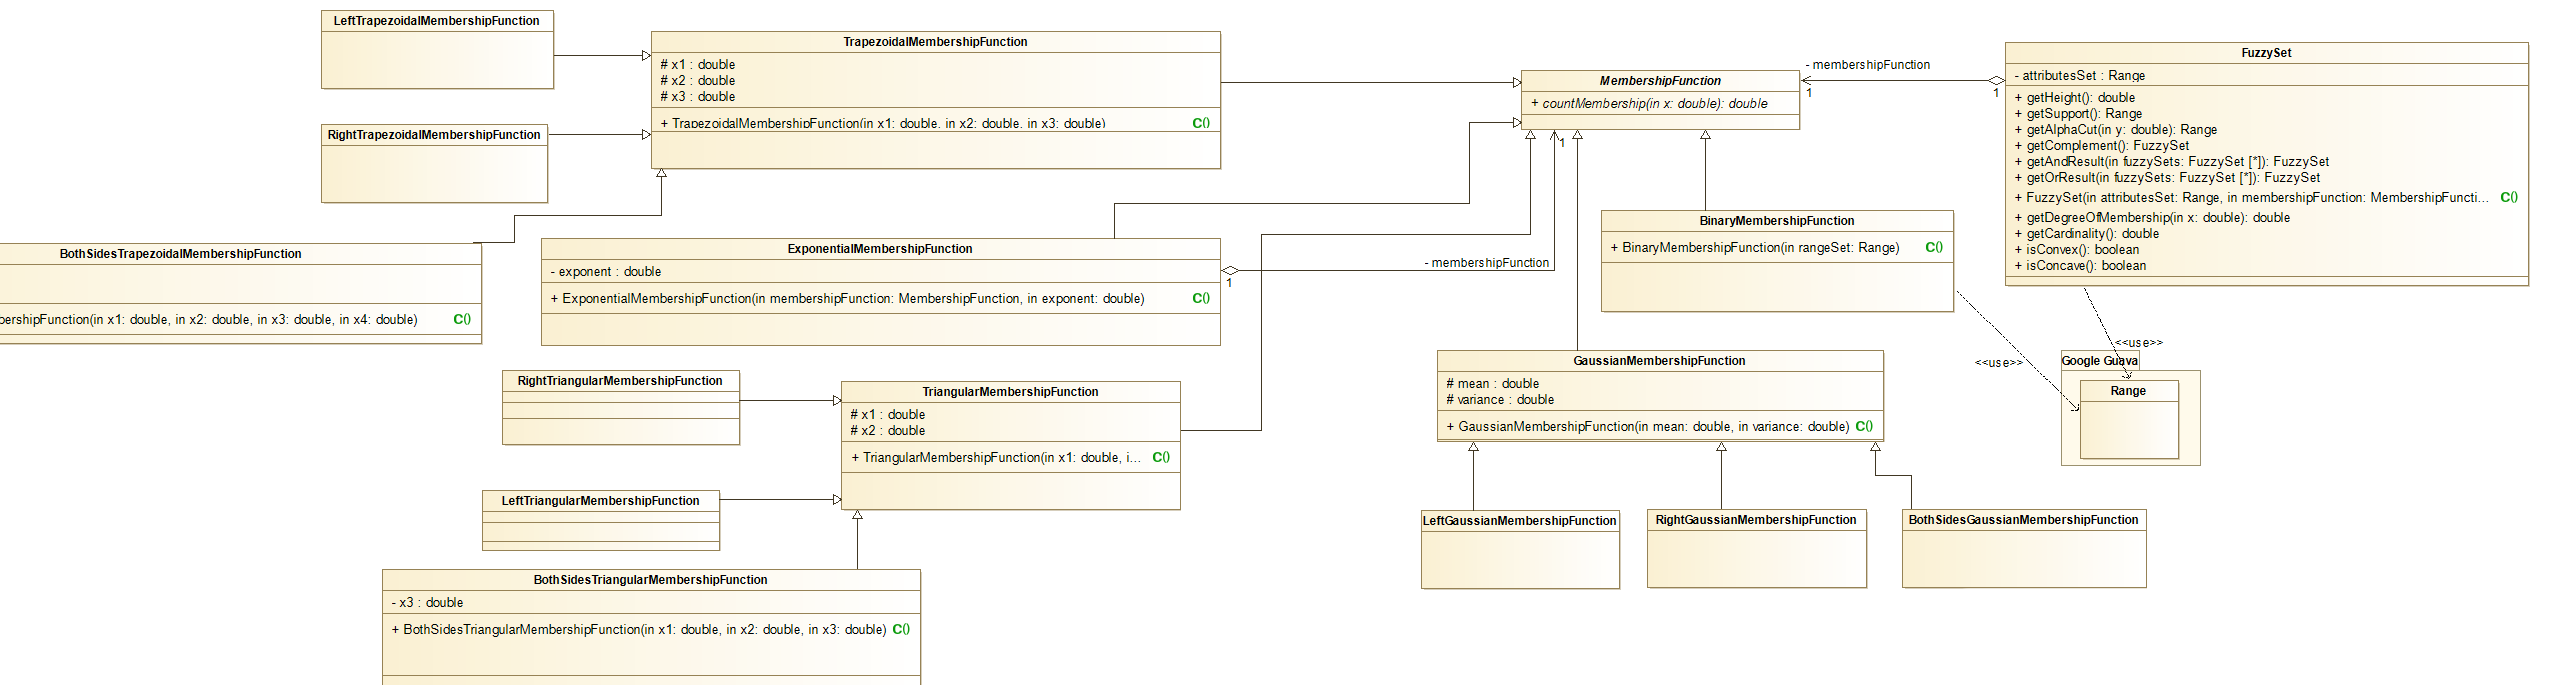
\includegraphics[width=14cm, height=5cm]{fuzzy_set_calculations.png}
    \caption{Diagram UML pakietu FuzzySetCalculations.}
    \label{rysunek:UML_fuzzy_set}
\end{figure}



\subsection{Diagram UML generatora podsumowań. Krótka instrukcja użytkownika} 

Drugim pakietem użytym przez nas w aplikacji jest pakiet generatora podsumowań. Składa się on z następujących elementów:
{\bf Label} - klasa reprezentująca pojedynczą etykietę. Etykieta zawiera swoją nazwę oraz pole odpowiadające za klasę \textit{FuzzySet}. Dzięki temu w etykiecie mamy dostęp do metod klasy \textit{FuzzySet}, w tym \textit{getDegreeOfMembership(double x)}, czyli stopień przynależności dla zadanego argumentu.

{\bf LingusticVariable} - klasa odpowiadająca za zmienną lingwistyczną. Posiada ona swoją nazwę oraz pole \textit{rangeSet}, które odpowiada za przestrzeń rozważań dla podanej zmiennej lingwistycznej. Poza tym klasa ta posiada pole typu Label, które odpowiada za wyżej wymienioną etykietę.

{\bf LinguisticQuantifier} - klasa abstrakcyjna reprezentująca kwantyfikator lingwistyczny. Kwantyfikator lingwistyczny posiada etykietę. Z klasy abstrakcyjnej \textit{LingusticQuantifier} dziedziczą dwie następujące klasy:
\begin{itemize}
    \item {\bf AbsoluteQuantifier} - kwantyfikator absolutny posiadający dodatkowo poza polami, które dziedziczy przedział rozważań.
    \item {\bf RelativeQuantifier} - kwantyfikator względny.
\end{itemize}

{\bf Player} - klasa z modułu DAO odpowiadającego za wczytywanie danych. Klasa ta odpowiada za pojedynczego zawodnika wczytanego z bazy danych.

{\bf LingusticSummariesGenerator} - klasa odpowiadająca za generowanie podsumowań, a w zasadzie pojedynczego podsumowania. Zawiera ona kwantyfikator lingwistyczny, pole typu Player, co odpowiada podmiotowi podsumowania. Klasa zawiera także pola: \textit{qualifier} (kwalifikator) oraz \textit{summarizer} (sumaryzator). Oba pola są Listami typów \textit{Label}. Klasa ta pozwala także oczywiście na wygenerowanie podsumowania.

{\bf QualityMeasures} - klasa zawierająca jedno pole - LinguisticSummariesGenerator. Klasa ta pozwala na obliczenie miar jakości od $T_1$ do $T_{11}$ \cite{niewiadomski19} dla wygenerowanego podsumowania.

\begin{figure}[H]
    \centering
    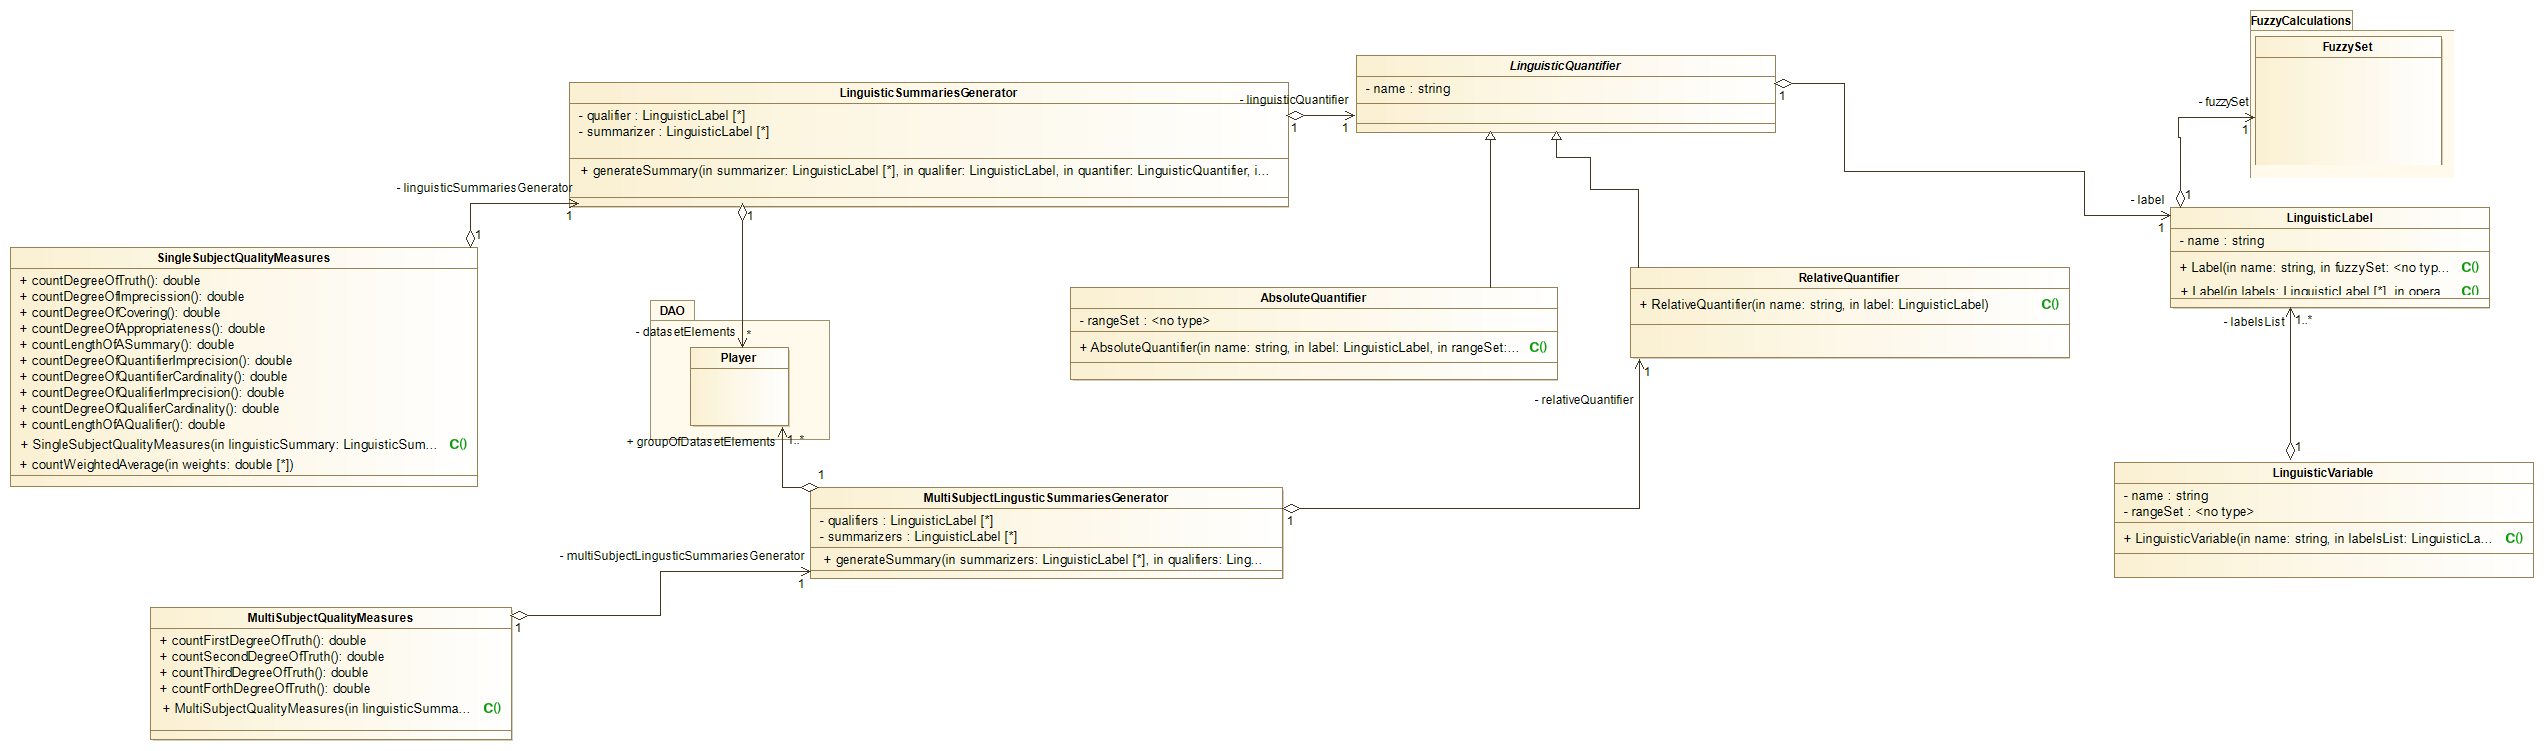
\includegraphics[width=14cm, height=5cm]{generator.png}
    \caption{Diagram UML generatora podsumowań.}
    \label{rysunek:generator}
\end{figure}

Po włączeniu aplikacji ukazuje nam się następujący ekran z podsumowaniami jednopodmiotowymi:
\begin{figure}[H]
    \centering
    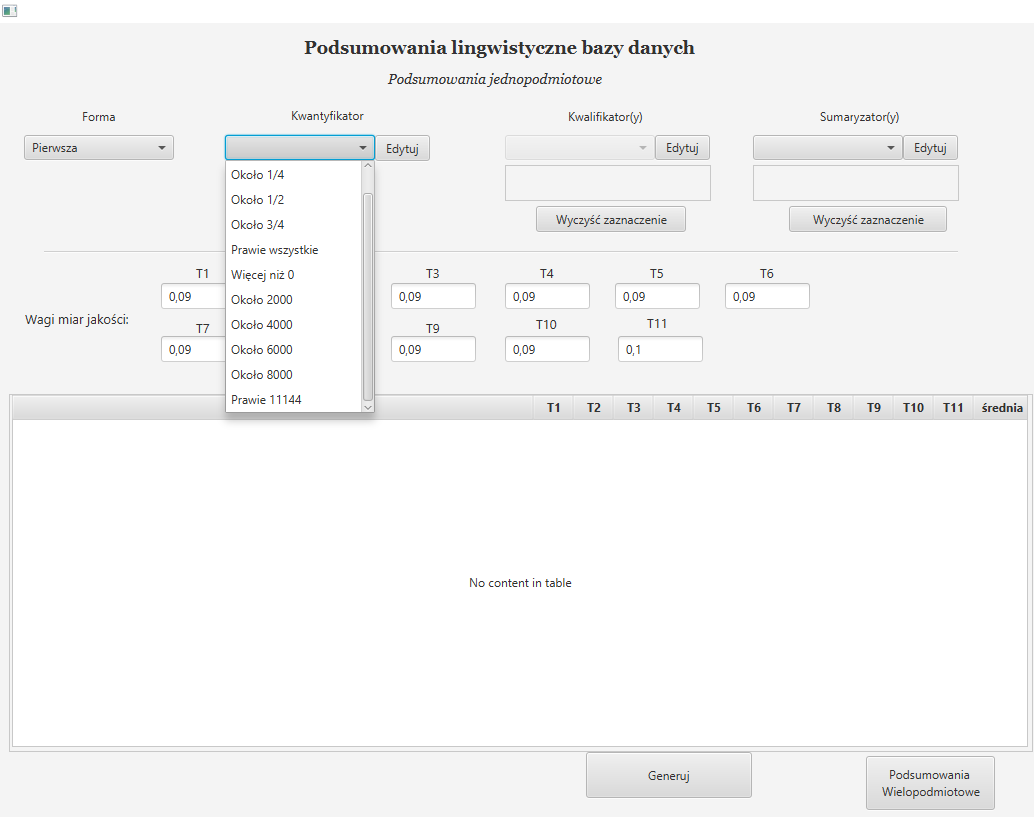
\includegraphics[width=14cm]{gui.png}
    \caption{Interfejs użytkownika po włączeniu aplikacji}
    \label{rysunek:gui}
\end{figure}
Na powyższym ekranie możemy wybrać odpowiednie interesujące nas wartości z rozwijalnych list. W przypadku wybrania formy pierwszej zablokowany jest wybór kwalifikatora (jako że w formie pierwszej podsumowań jednopododmiotowych nie występują kwalifikatory), a do wyboru mamy wszystkie kwantyfikatory (zarówno absolutne, jak i względne). W przypadku formy drugiej możemy wybrać kwalifikatory, a do wyboru w przypadku kwantyfikatorów są tylko kwantyfikatory względne. Zarówno w przypadku kwalifikatorów i sumaryzatorów możemy wybrać więcej niż jedną etykietę, które to będą połączone spójnikiem "i". Przyciski "Wyczyść zaznaczenie" czyszczą nam listę wybranych sumaryzatorów i kwalifikatorów. Po naciśnięciu przycisku "Edytuj" zostajemy przeniesieni do okna umożliwiającego edycje i definiowanie nowych etykiet. Poniżej okna z etykietami od T1 do T11 oznaczają wagi dla poszczególnych miar, które zostaną użyte przy liczeniu miary podsumowania optymalnego. Przycisk "Generuj" generuje nam podsumowanie, które to pojawia się w przewijalnej tabeli. W tabeli możliwe jest sortowanie po konkretnej mierze. Kolumna z etykietą "średnia" oznacza miarę podsumowania optymalnego. Przycisk "Podsumowania Wielopodmiotowe" przenosi nas do okna z podsumowaniami wielopodmiotowymi.Tam, analogicznie to podsumowań jednopodmiotowych przy wybraniu formy podsumowania zostają zablokowane/odblokowane poszczególne możliwości wyboru kwalifikatrów/sumaryzatorów. Cała reszta również jest analogiczna do podsumowań jednopodmiotowych, poza wagami. Dla podsumowań wielopodmiotowych liczymy jedynie jedną miarę, zatem nie ma możliwości przypisywania wag.
\\
Aplikacja została napisana przy użyciu Java 11 \cite{java_doc}, Apache Maven \cite{maven_doc}, oraz JavaFX 13 \cite{javafx_doc}. Aby uruchomić aplikację należy załadować projekt mavenowy, a następnie wykonać polecenie mvn install. Możemy to zrobić z konsoli, bądź wykorzystując do tego IDE (np. IntelliJ i pasek rozwijalny po prawej stronie). Kolejnym krokiem jest uruchomienie wtyczki javafx, bądź exec, poprzez przejście do folderu z modułem GUI i wykonanie polecenia mvn javafx:run, bądź mvn exec:java. Możemy to zrobić także przy użyciu IDE. Spowoduje to wyświetlenie interfejsu użytkownika i umożliwi korzystanie z aplikacji.

\section{ Jednopodmiotowe podsumowania lingwistyczne. Miary jakości, podsumowanie optymalne}

We wszystkich przedstawionych poniżej eksperymentach kolumna z nazwą "średnia" oznacza miarę jakości podsumowania optymalnego.

\subsection{Jednopodmiotowe podsumowania lingwistyczne w formie pierwszej}

Dla jednopodmiotowych podsumowań lingwistycznych w formie pierwszej przeprowadziliśmy dwa eksperymenty, w każdym z nich przyjmując inne wagi. Wyniki dla eksperymentu nr 1 prezentują się następująco:

\begin{figure}[H]
    \centering
    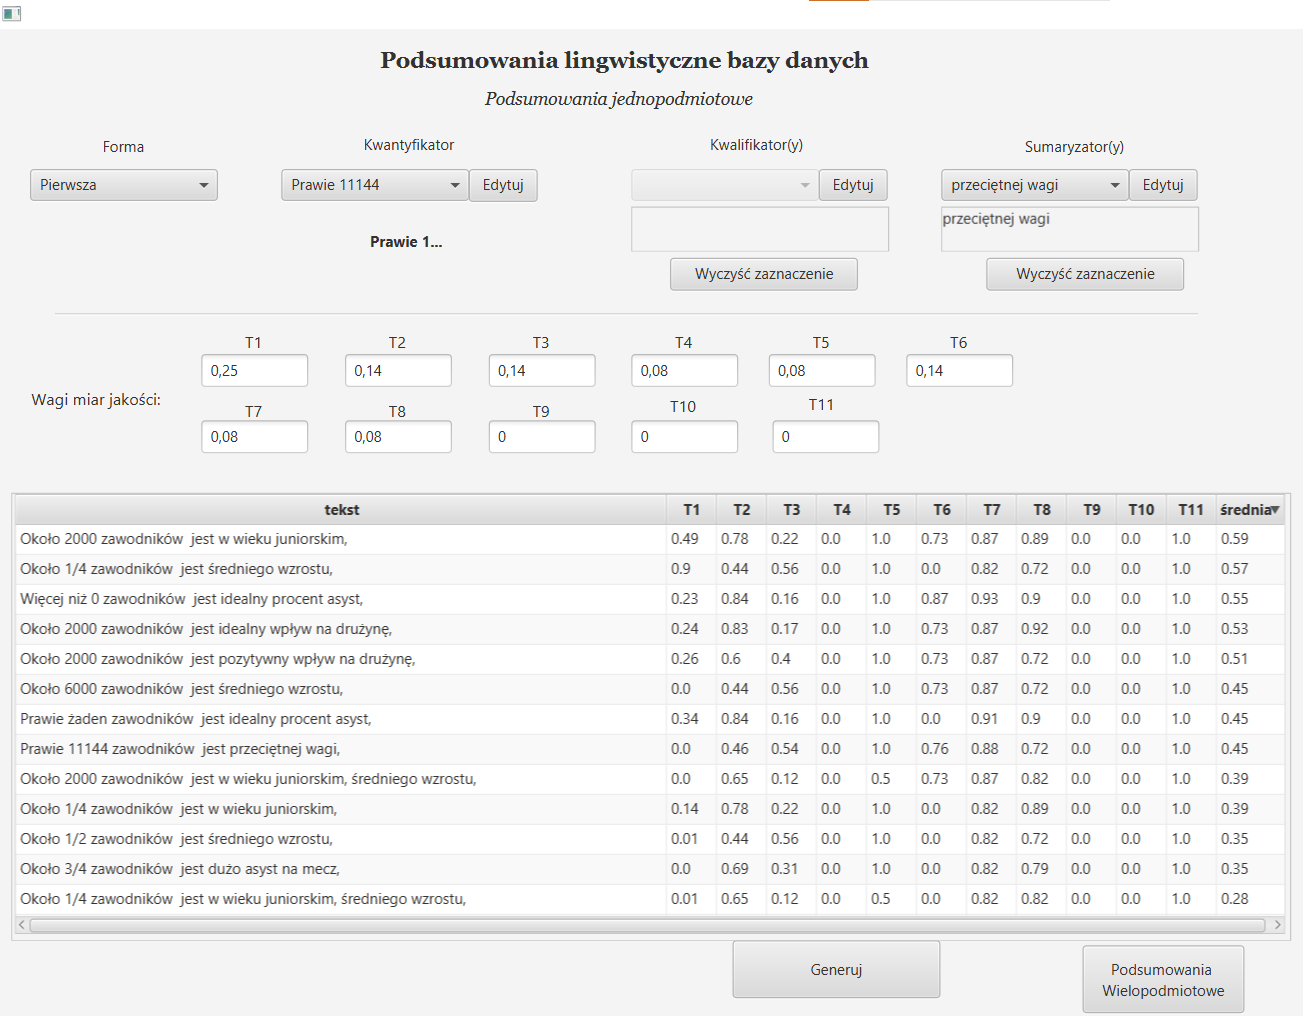
\includegraphics[width = 14cm]{eksperyment1.png}
    \caption{Wyniki eksperymentu nr 1 dla jednopodmiotowych podsumowań lingwistycznych w formie pierwszej}
    \label{rysunek:forma_pierwsza_eksperyment_1}
\end{figure}

Podsumowanie "Około 2000 zawodników jest w wieku juniorskim" osiągnęło najwyższą wartość miary jakości podsumowania optymalnego porównując z innymi podsumowaniami wygenerowanymi w tym eksperymencie. Wyniosła ona 0.59. Warto zauważyć, że w tym wypadku dodając kolejny sumaryzator jakość podsumowania maleje ("Około 1/4 zawodników jest średniego wzrostu" znajduje się na liście na pozycji drugiej, "Około 1/4 zawodników jest w wieku juniorskim" na pozycji 10, natomiast podsumowanie "Około 1/4 zawodników jest w wieku juniorskim, średniego wzrostu" dopiero na pozycji 13. Najwyższą wartość miary T1 osiągnęło podsumowanie "Około 1/4 zawodników jest średniego wzrostu", jednak biorąc pod uwagę miarę podsumowania optymalnego podsumowanie to znajduje się na 2 miejscu. Warto zwrócić uwagę na miarę T6, która lekko zakłamuje nam obraz. Dla kwantyfikatora względnego miara ta w każdym przypadku pokazuje 0. Wynika to z tego, że ten typ kwantyfikatorów wyraża się w tym wypadku funkcją Gaussowską, która to dąży do zera (jednak wartości 0 nie przyjmuje)
\\
W kolejnym eksperymencie zmodyfikowaliśmy nieco wagi średnich, a jego wyniki prezentują się następująco: 
\begin{figure}[H]
    \centering
    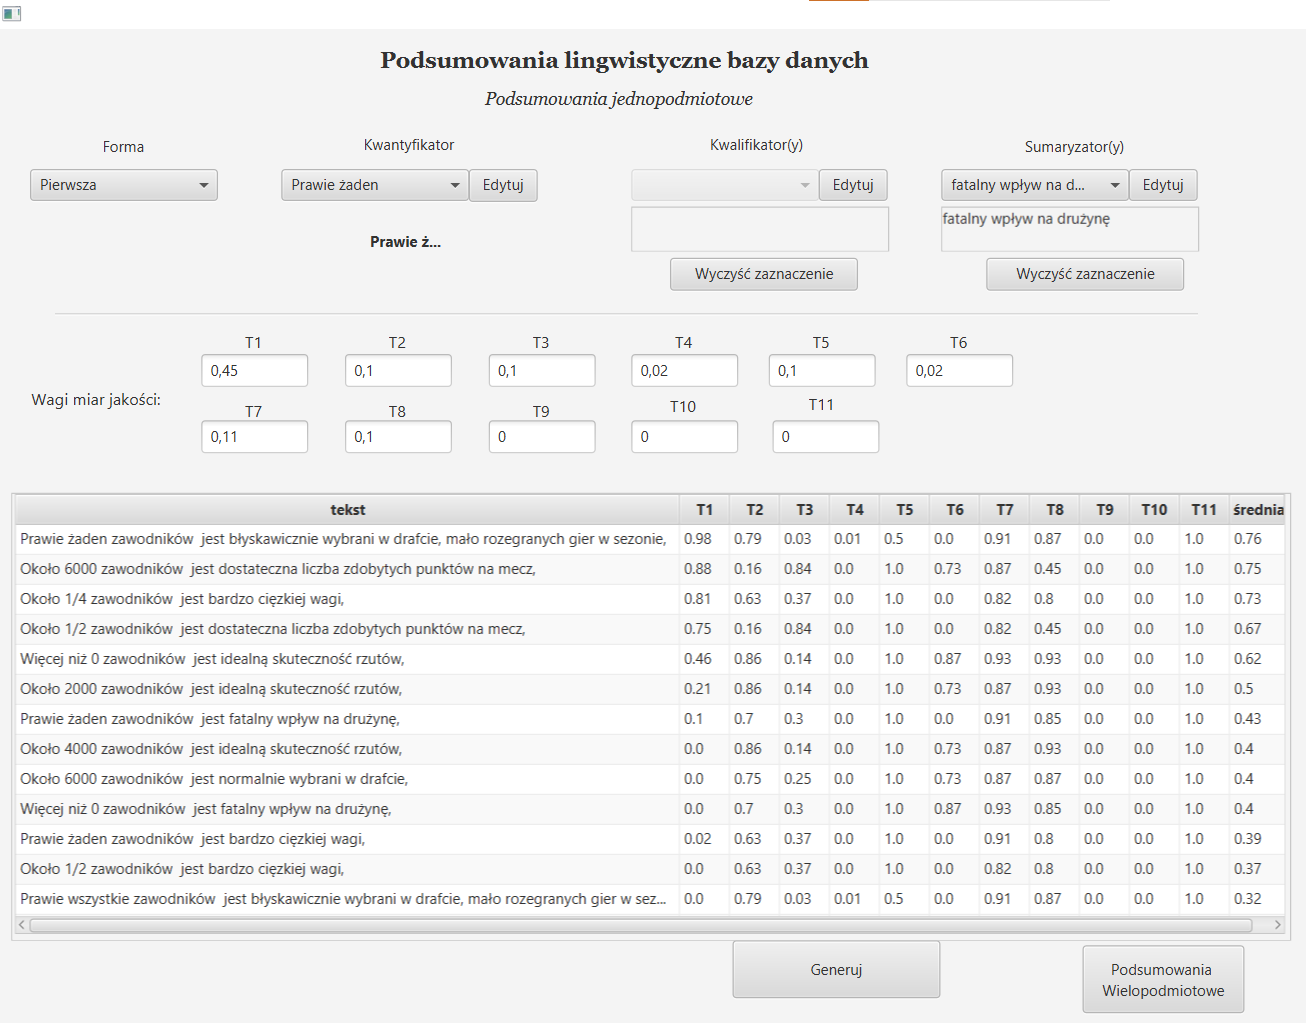
\includegraphics[width = 14cm]{eksperyment2.png}
    \caption{Wyniki eksperymentu nr 2 dla jednopodmiotowych podsumowań lingwistycznych w formie pierwszej}
    \label{rysunek:forma_pierwsza_eksperyment_2}
\end{figure}
W tym eksperymencie zmieniliśmy wagi, w sczególności zwiększając wagę dla miary T1 oraz zmniejszając wagę dla miary T6. Najlepszym podsumowaniem w tym eksperymencie okazało się "Prawie żaden zawodnik jest błyskawicznie wybrany w drafcie i ma ma mało rozegranych gier w sezonie [0.76]". Jest to jak najbardziej logiczne, ponieważ kluby wybierają zawodników w drafcie szybko, aby ci stanowili o sile ich drużyny. Podsumowanie to osiągnęło wartość T1 aż na poziomie 0.98. Jak widzimy, przy takim dobraniu wag jak powyżej byliśmy w stanie zminimalizować negatywny wpływ funkcji gaussowskiej na ostateczny wynik miary jakości podsumowania optymalnego. Zarówno w tym jak i w poprzednim eksperymencie przyjęliśmy wagi dla T9, T10 i T11 na 0, ponieważ miary te dotyczą kwalifikatorów, których w formie pierwszej podsumowań jednopodmiotowych nie ma.
\subsection{Jednopodmiotowe podsumowania lingwistyczne w formie drugiej}

Dla formy drugiej jednopodmiotowych podsumowań lingwistycznych przeprowadziliśmy 1 eksperyment, którego wyniki przedstawiają się następująco:
\begin{figure}[H]
    \centering
    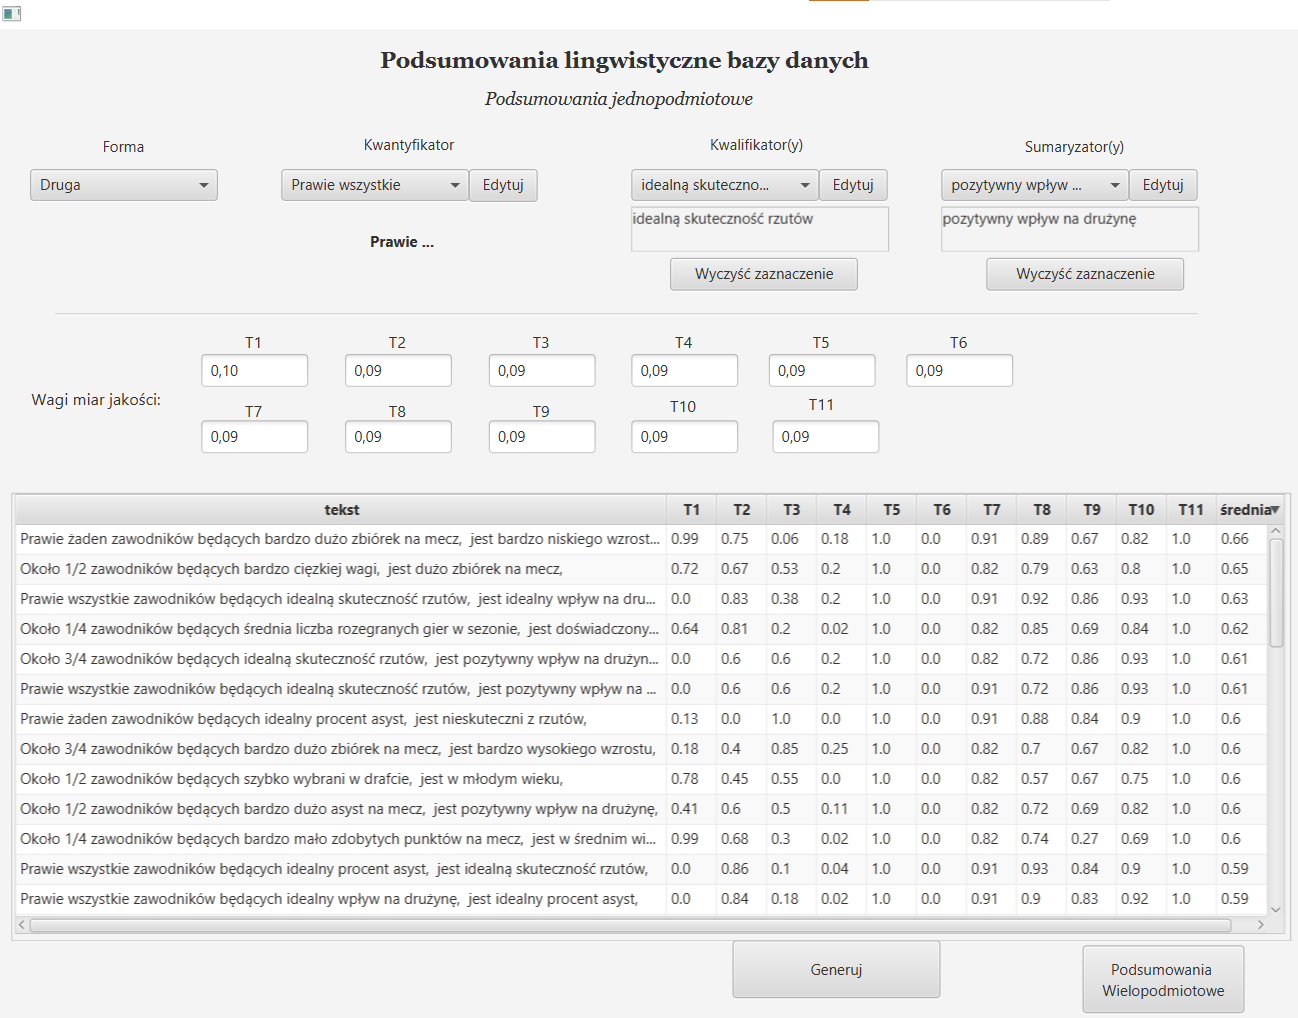
\includegraphics[width = 14cm]{eksperyment3.png}
    \caption{Wyniki eksperymentu nr 1 dla jednopodmiotowych podsumowań lingwistycznych w formie drugiej}
    \label{rysunek:forma_druga_eksperyment_1}
\end{figure}

Tym razem wagi rozłożyliśmy równomiernie. Najlepszym podsumowaniem sortując po mierze podsumowania optymalnego okazało się "Prawie żaden zawodnik mający bardzo dużo zbiórek na mecz, jest bardzo niskiego wzrostu [0.66]" Podsumowanie to osiągnęło wartość miary T1 (stopień prawdziwości) aż 0,99. Stopień prawdziwości 0,99 osiągnęło także podsumowanie "Około 1/4 zawodników mających bardzo mało zdobytych punktów na mecz, jest w średnim wieku [0.60]". Końcowa miara dla tego podsumowania wyniosła 0.60. Wysoką wartość miary podsumowania optymalnego (0.65) uzyskało także podsumowanie "Około 1/2 zawodników będących bardzo ciężkiej wagi, ma dużo zbiórek na mecz.



\section{Wielopodmiotowe podsumowania lingwistyczne i~ich miary jakości} 
Wyniki kolejnych eksperymentów wg punktów 2.-4. opisu projektu 2. Uzasadnienie i
metoda podziału zbioru danych na rozłączne podmioty. Listy podsumowań
wielopodmiotowych i tabele/rankingi podsumowań dla danych atrybutów obowiązkowe i
dokładnie opisane w ,,captions'' (tytułach), konieczny opis kolumn i wierszy tabel.
Konieczne uwzględnienie wszystkich 4-ch form podsumowań wielopodmiotowych. 
\\ 

** Możliwe sformułowanie zagadnienia wielopodmiotowego podsumowania optymalnego **.\\

{**Ewentualne wyniki realizacji punktu ,,na ocenę 5.0'' wg opisu Projektu 2. i ich porównanie do wyników z
części obowiązkowej**.}\\

\noindent {\bf Sekcja uzupełniona jako efekt zadania Tydzień 12 wg Harmonogramu Zajęć
na WIKAMP KSR.}


\section{Dyskusja, wnioski}
\subsection{Jednopodmiotowe podsumowania lingwistyczne w formie pierwszej}

W mierze T6, w której pod uwagę bierzemy nośnik kwantyfikatora niezwykle ważny jest typ funkcji przynależności dla kwantyfikatora. Dla funkcji Gaussowskiej miara ta zawsze przyjmowała będzie wartość 0, ponieważ wykres funkcji Gaussa na całej przestrzeni rozważań nie przyjmuje wartości 0. Łącząc sumaryzatory, których połączenie wydaje nam się logiczne i które wydają się w jakiś sposób skorelowane ze sobą(jak np. "błyskawicznie wybrany w drafcie" i "mało rozegranych gier w sezonie") otrzymujemy podsumowania o bardzo wysokiej mierze T1, a więc stopniu prawdziwości. Warto zauważyć, że dla tego samego kwantyfikatora zmieniając tylko sumaryzatory, bądź dla tych samych sumaryzatorów zmieniając tylko kwantyfikatory tylko niektóre z miar zmieniają swoje wartości. Oznacza to po prostu, że część miar zależy tylko i wyłącznie od sumaryzatora/kwantyfikatora, nie łącząc tych dwóch zbiorów rozmytych ze sobą, stąd tak ważna jest analiza wszystkich miar przy wyciąganiu wniosków.

\subsection{Jednopodmiotowe podsumowania lingwistyczne w formie drugiej}
Z podsumowań jednopodmiotowych w formie drugiej płynie więcej wniosków dotyczących zbioru danych zawodników koszykówki. Możemy bowiem wywnioskować chociażby, że zawodnicy bardzo niskiego wzrostu nie przewodzą w statystykach jeśli chodzi o zbiórki. Natomiast zawodnicy ważący bardzo dużo często zaliczają dużo zbiórek na mecz. Poza tym możemy wywnioskować, że około połowy zawodników wybranych szybko w drafcie są aktualnie w młodym wieku. Możemy z tego zdania wysnuć wniosek, że zawodnicy wybrani w drafcie szybko początkowe lata grają w NBA, jednak potem ze różnych względów odchodzą z najbardziej prestiżowej ligi koszykówki świata. Jeśli chodzi oo wnioski dotyczące miar płynące z tej części eksperymentów to zdecydowanie było w nich widać, że im więcej nie powiązanych ze sobą kwalifikatorów/sumaryzatorów użyjemy tym podsumowanie jest gorszej jakości. Można także zauważyć, że miara T7 jest podobna dla wszystkich podsumowań. Świadczy to o tym, że kwantyfikatory są równomiernie rozłożone - ich pola pod wykresami są podobne. Zauważamy także, że miary T9, T10 i T11, czyli miary zależące od kwalifikatorów przyjmują w większości przypadków duże wartości. Świadczy to o tym, że kwalifikatory w formie drugiej podsumowań jednopodmiotowych zostały dobrane odpowiednio.\\

Dokładne interpretacje uzyskanych wyników w zależności od parametrów klasyfikacji
opisanych w punktach 3.-4 opisu Projektu 2. 
Szczególnie istotne są wnioski o charakterze uniwersalnym, istotne dla podobnych zadań. 
Omówić i wyjaśnić napotkane problemy (jeśli były). Każdy wniosek/problem powinien mieć poparcie
w przeprowadzonych eksperymentach (odwołania do konkretnych wyników: tabel i miar
jakości). Ocena które wybrane kwantyfikatory, sumaryzatory, kwalifikatory i/lub ich
miary jakości mają małe albo duże znaczenie dla wiarygodności i jakości otrzymanych
agregacji/podsumowań.  \\
\underline{Dla końcowej oceny jest to najważniejsza sekcja} sprawozdania, gdyż prezentuje poziom
zrozumienia rozwiązywanego problemu.\\

** Możliwości kontynuacji prac w obszarze logiki rozmytej i wnioskowania rozmytego, zwłaszcza w kontekście pracy inżynierskiej,
magisterskiej, naukowej, itp. **\\

\noindent {\bf Sekcja uzupełniona jako efekt zadań Tydzień 11 i Tydzień 12 wg
Harmonogramu Zajęć na WIKAMP KSR.}


\section{Braki w realizacji projektu 2.}
Wymienić wg opisu Projektu 2. wszystkie niezrealizowane obowiązkowe elementy projektu, ewentualnie
podać merytoryczne (ale nie czasowe) przyczyny tych braków. 


\begin{thebibliography}{99}
 \bibitem{niewiadomski19} A. Niewiadomski, Zbiory rozmyte typu 2. Zastosowania w reprezentowaniu informacji.  Seria „Problemy współczesnej informatyki” pod redakcją L. Rutkowskiego. Akademicka Oficyna Wydawnicza EXIT, Warszawa, 2019.
\bibitem{zadrozny06} S. Zadrożny, Zapytania nieprecyzyjne i lingwistyczne podsumowania baz danych, EXIT, 2006, Warszawa
\bibitem{niewiadomski08} A. Niewiadomski, Methods for the Linguistic Summarization of Data: Applications of Fuzzy Sets and Their Extensions, Akademicka Oficyna Wydawnicza EXIT, Warszawa, 2008.
\bibitem{nba_data} Baza danych zawierająca statystyki koszykarzy z ligi NBA z lat 1996-2020 [przeglądany 04.05.2021] Dostępna w:
https://www.kaggle.com/justinas/nba-players-data
\bibitem{uml_doc} Dokumentacja diagramów UML [przeglądana 24.05.2021] Dostępna w:
https://www.uml-diagrams.org/
\bibitem{java_doc} Dokumentacja Java 11 [przeglądana 03.06.2021] Dostępna w: https://docs.oracle.com/en/java/javase/11/
\bibitem{maven_doc} Dokumentacja Maven [przeglądana 03.06.2021] Dostępna w: https://maven.apache.org/guides/
\bibitem{javafx_doc} Dokumentacja JavaFx 13 [przeglądana 03.06.2021] Dostępna w: https://openjfx.io/javadoc/13/
\end{thebibliography}

Literatura zawiera wyłącznie źródła recenzowane i/lub o potwierdzonej wiarygodności,
możliwe do weryfikacji i cytowane w sprawozdaniu. 
\end{document}
